%% History:
%% May 2019 Tomi Männistö, Antti-Pekka Tuovinen proofreading; 30 vs. 40 cr theses, etc.
%% May 2019 Tomi Männistö changed from babelbib to bibtex; Abstract page (and other pages as well) reformatting.
%% January–May 2019 several issues fixed by Niko Mäkitalo; long fields in abstract
%% March 2018 template file extended by Lea Kutvonen to exploit HYthesisML.cls.
%% Feb2018 This template file for the use of HYgraduML.cls was  modified by Veli Mäkinen from HY_fysiikka_LuKtemplate.tex
%% authored by Roope Halonen ja Tomi Vainio in 2017.
%% Some text is also inherited from engl_malli.tex versions by Kutvonen, Erkiö, Mäkelä, Verkamo, Kurhila, and
%% Nykänen, to accompany tktltiki.cls (by Puolakka 2002).


%% Follow comments to support use.

%%%%%%%%%%%%%%%%%%%%%%%%%%%%%%%%%%%%%%%%%%%%%%%%%%%%%%%%%
%% STEP 1: Choose options for MSc / BSc layout and your bibliographic style
%%%%%%%%%%%%%%%%%%%%%%%%%%%%%%%%%%%%%%%%%%%%%%%%%%%%%%%%%

%%  Language: 
%%      finnish, swedish, or english
%%  Pagination (use twoside by default)  
%%      oneside or twoside,
%%  Study programme / kind of report
%%      csm  = pro gradu in new Computer science MSc;
%%      cs = pro gradu in old Computer Science MSc;
%%      tkt = BSc thesis in new curricula;
%%      tktl= BSc thesis in old curricula;
%%  For MSc choose your line or track:
%%      (30 cr thesis, 2020 onwards, Master of Computer Science programme = csm)
%%      software-track-2020 = Software study track
%%      algorithms-track-2020 = Algorithms study track
%%      networking-track-2020 = Networking study track
%%
%%      (30 cr thesis, Master of Computer Science programme = csm)
%%      sw-track-2018 = Software Systems study track
%%      alko-track-2018 = Algorithms study track
%%      nodes-track-2018 = Networking and Services study track
%%
%%      (30 cr thesis, Master of Computer Science programme = csm)
%%      sw-line-2017 =  Software systems subprogramme
%%      alko-line-2017 = Algorithms, Data Analytics and Machine Learning subprogramme
%%      bio-line-2017 = Algorithmic Bioinformatics subprogramme
%%      nodes-line-2017 = Networking and Services subprogramme
%%
%%      (40 cr thesis, = cs)
%%      sw-line = Software Systems specialisation line 
%%      alko-line = Algorithms specialisation line
%%      bio-line = Algorithmic bioinformatics specialisation line
%%      nodes-line = Networking and Services specialisation line

\documentclass[english,twoside,censored,csm,algorithms-track-2020]{HYthesisML}


% In theses, open new chapters only at right page.
% For other types of documents, may ask "openany" in document.
\PassOptionsToClass{openright,twoside,a4paper}{report}
%\PassOptionsToClass{openany,twoside,a4paper}{report}

\usepackage{csquotes}
%%%%%%%%%%%%%%%%%%%%%%%%%%%%%%%%%%%%%%%%%%%%%%%%%%%%%%%%%
%% REFERENCES
%% Some notes on bibliography usage and options:
%% natbib -> you can use, e.g., \citep{} or \parencite{} for (Einstein, 1905); with APA \cite -> Einstein, 1905 without ()
%% maxcitenames=2 -> only 2 author names in text citations, if more -> et al. is used
%% maxbibnames=99 as no great need to suppress the biliography list in a thesis
%% for more information see biblatex package documentation, e.g., from https://ctan.org/pkg/biblatex 

%% Reference style: select one 
%% for APA = Harvard style = authoryear -> (Einstein, 1905) use:
\usepackage[style=authoryear,bibstyle=authoryear,backend=biber,natbib=true,maxnames=99,maxcitenames=2,giveninits=true,uniquename=init]{biblatex}
%% for numeric = Vancouver style -> [1] use:
%\usepackage[style=numeric,bibstyle=numeric,backend=biber,natbib=true,maxbibnames=99,giveninits=true,uniquename=init]{biblatex}
%% for alpahbetic -> [Ein05] use:
%\usepackage[style=alphabetic,bibstyle=alphabetic,backend=biber,natbib=true,maxbibnames=99,giveninits=true,uniquename=init]{biblatex}
%

\addbibresource{bibliography.bib}
% in case you want the final delimiter between authors & -> (Einstein & Zweistein, 1905) 
% \renewcommand{\finalnamedelim}{ \& }
% List the authors in the Bibilipgraphy as Lastname F, Familyname G,
\DeclareNameAlias{sortname}{family-given}
% remove the punctuation between author names in Bibliography 
%\renewcommand{\revsdnamepunct}{ }


%% Block of definitions for fonts and packages for picture management.
%% In some systems, the figure packages may not be happy together.
%% Choose the ones you need.

%\usepackage[utf8]{inputenc} % For UTF8 support, in some systems. Use UTF8 when saving your file.

\usepackage{lmodern}         % Font package, again in some systems.
\usepackage{textcomp}        % Package for special symbols
\usepackage[pdftex]{color, graphicx} % For pdf output and jpg/png graphics
\usepackage{epsfig}
\usepackage{subfigure}
\usepackage{algorithm}
\usepackage[algo2e]{algorithm2e}
\usepackage[]{algpseudocode}
\usepackage[pdftex, plainpages=false]{hyperref} % For hyperlinks and pdf metadata
\usepackage{fancyhdr}        % For nicer page headers
\usepackage{tikz}            % For making vector graphics (hard to learn but powerful)
%\usepackage{wrapfig}        % For nice text-wrapping figures (use at own discretion)
\usepackage{amsmath, amssymb} % For better math

\singlespacing               %line spacing options; normally use single

\fussy
%\sloppy                      % sloppy and fussy commands can be used to avoid overlong text lines
% if you want to see which lines are too long or have too little stuff, comment out the following lines
% \overfullrule=1mm
% to see more info in the detailed log about under/overfull boxes...
% \showboxbreadth=50 
% \showboxdepth=50



%%%%%%%%%%%%%%%%%%%%%%%%%%%%%%%%%%%%%%%%%%%%%%%%%%%%%%%%%
%% STEP 2:
%%%%%%%%%%%%%%%%%%%%%%%%%%%%%%%%%%%%%%%%%%%%%%%%%%%%%%%%%
%% Set up personal information for the title page and the abstract form.
%% Replace parameters with your information.
\title{Multi-task learning in Computer Vision}

% TM: Contributors to template editors now listed in the beginning of the file in comments
\author{Konsta Kutvonen}
\date{\today}



% Set supervisors and examiners, use the titles according to the thesis language
% Prof. 
% Dr. or in Finnish toht. or tri or FT, TkT, Ph.D. or in Swedish... 
\supervisors{Associate Professor Laura Ruotsalainen}
\examiners{Associate Professor Laura Ruotsalainen, Professor Jyrki Kivinen } 


\keywords{computer vision, deep learning, convolutional neural networks, multi-task learning}
\additionalinformation{\translate{\track}}

%% For seminar papers and such, cover page and abstract
%% requires these three basic items of information.
%% Label as needed and remove comment marks.
%%\level{Seminaariraportti}
%%\programme{Tietojenkäsittelytieteen andidaattiohjelma}
%%\subject{Seminaarisarjan nimi}

%% Replace classification terms with the ones that match your work. ACM
%% ACM Digital library provides a taxonomy and a tool for classification
%% in computer science. Use 1-3 paths, and use right arrows between the
%% about three levels in the path; each path requires a new line.

\classification{\protect{\ \\
\  Computing methodologies $\rightarrow$ Artificial intelligence  $\rightarrow$ Computer vision \  \\
\  Computing methodologies $\rightarrow$ Machine learning  $\rightarrow$ Learning paradigms $\rightarrow$ Multi-task learning
}}

%% if you want to quote someone special. You can comment this line out and there will be nothing on the document.
%\quoting{Bachelor's degrees make pretty good placemats if you get them laminated.}{Jeph Jacques}


%% OPTIONAL STEP: Set up properties and metadata for the pdf file that pdfLaTeX makes.
%% Your name, work title, and keywords are recommended.
\hypersetup{
    unicode=true,           % to show non-Latin characters in Acrobat’s bookmarks
    pdftoolbar=true,        % show Acrobat’s toolbar?
    pdfmenubar=true,        % show Acrobat’s menu?
    pdffitwindow=false,     % window fit to page when opened
    pdfstartview={FitH},    % fits the width of the page to the window
    pdftitle={Multi-task learning in Computer Vision},            % title
    pdfauthor={Konsta Kutvonen},           % author
    pdfsubject={},          % subject of the document
    pdfcreator={},          % creator of the document
    pdfproducer={pdfLaTeX}, % producer of the document
    pdfkeywords={something} {something else}, % list of keywords for
    pdfnewwindow=true,      % links in new window
    colorlinks=true,        % false: boxed links; true: colored links
    linkcolor=black,        % color of internal links
    citecolor=black,        % color of links to bibliography
    filecolor=magenta,      % color of file links
    urlcolor=cyan           % color of external links
}

%%-----------------------------------------------------------------------------------

\begin{document}

% Generate title page.
\maketitle


%%%%%%%%%%%%%%%%%%%%%%%%%%%%%%%%%%%%%%%%%%%%%%%%%%%%%%%%%
%% STEP 3:
%%%%%%%%%%%%%%%%%%%%%%%%%%%%%%%%%%%%%%%%%%%%%%%%%%%%%%%%%
%% Write your abstract to be positioned here.
%% You can make several abstract pages (if you want it in different languages),
%% but you should also then redefine some of the above parameters in the proper
%% language as well, in between the abstract definitions.

\begin{otherlanguage}{english}
    \begin{abstract}
        With modern computer vision algorithms, it is possible to solve many different kinds of problems, such as image detection, image classification, and image segmentation.
        In some cases, like in the case of a camera-based self-driving car, the task can't yet be adequately solved as a direct mapping from image to action with a single model.
        In such situations, we need more complex systems that can solve multiple computer vision tasks to understand the environment and act based on it for acceptable results.
        Training each task on their own can be expensive in terms of storage required for all weights and especially for the inference time as the output of several large models is needed.
        Fortunately, many state-of-the-art solutions to these problems use Convolutional Neural Networks and often feature some ImageNet backbone in their architecture.
        With multi-task learning, we can combine some of the tasks into a single model, sharing the convolutional weights in the network.
        Sharing the weights allows for training smaller models that produce outputs faster and require less computational resources, which is essential, especially when the models are run on embedded devices with constrained computation capability and no ability to rely on the cloud. 
        
        In this thesis, we will present some state-of-the-art models to solve image classification and object detection problems.
        We will define multi-task learning, how we can train multi-task models, and take a look at various multi-task models and how they exhibit the benefits of multi-task learning.
        Finally, to evaluate how training multi-task models changes the basic training paradigm and to find what issues arise, we will train multiple multi-task models.
        The models will mainly focus on image classification and object detection using various data sets.
        They will combine multiple tasks into a single model, and we will observe the impact of training the tasks in a multi-task setting.
        
    \end{abstract}
\end{otherlanguage}

% Place ToC
\newpage
\mytableofcontents
\frontmatter

%%%%%%%%%%%%%%%%%%%%%%%%%%%%%%%%%%%%%%%%%%%%%%%%%%%%%%%%%
%% STEP 4: Write the thesis.
%%%%%%%%%%%%%%%%%%%%%%%%%%%%%%%%%%%%%%%%%%%%%%%%%%%%%%%%%
%% Your actual text starts here. You shouldn't mess with the code above the line except
%% to change the parameters. Removing the abstract and ToC commands will mess up stuff.
%%
%% You may wish to include material to avoid browsing the definitions
%% above. Command \include{file} includes the file of name file.tex.
%% As a side effect, subsequent inclusions may force a page break.

% BSc instructions
%\include{bsc_finnish_contents}
%
\chapter{Introduction}


In all writing for publication, the writer's freedom of creation and expression are limited by a number of guidelines and specific regulations.

At best, a familiar set of regulations shared by reader and writer can create a kind of support network that allows the message to be relayed without distortion. It will be easier for readers to find 
the pertinent contents in a piece of writing if its layout and structure are the same as they are used to. This also applies to writers. When writers follow a set presentation model, 
they do not have to waste time on considerations that are secondary to the work itself, but they can concentrate on polishing the contents of the text. This means that it is a good 
idea to practice following the rules for the layout, though you may think you know how to select a better way to present your work.

This is a guide for the layout and structure of theses and essays at the Department of Computer Science at the University of Helsinki. It is thus applicable to the course 
Scientific Writing, the software engineering projects, seminars, and MSc theses. (This is an updated version of 
the previous guide written by the course lecturers \citep{erkio01, erkiomakela96, erkio94, verkamo92}.)

The \LaTeX\ guide and \LaTeX\ style that has been  published on the department's web site can be used as support for this guide.


\chapter{Structure}

Let us start by looking at the sections expected to be in a scientific text. Keep in mind that the same expectations go for all kinds of technical writing.
However, this document in itself, is not a scientific or a research
text, so there will be content lacks in terms of research question
setting in the introduction and evaluative material in the last sections.

\section{Abstract or summary}
%\enlargethispage{5mm}


The summary page contains the following elements: the bibliographical data of the work, an abstract, topic classification, 
and the key words. The bibliographical data consists of title, name of the author, place of publication, date of publication, and number of pages.

The abstract should be short, generally one paragraph (100 words maximum) explaining the main contents of the work: topic, methodology and results.


 Topics are classified according to the ACM Computing Classification System
(CCS). A small set of paths (1-3) should be used, starting from any top nodes
referred to bu the root term CCS leading to the leaf nodes. The elements
in the path are separated by right arrow, and emphasis of each element individually can be indicated
by the use of bold face for high importance or italics for intermediate
level. The combination of individual boldface terms may give the reader
additional insight. 

\section{Introduction}


The purpose of the introduction is to introduce the goals of the work in general terms. Describe topic, 
methodology and results (as in the abstract, but expand it).
In order to provide the reader a good starting point for
interpretations, it is good to start the introduction by
contextualisation of the challenges and solutions to be discussed. For
example, why a certain domain has a particular challenge and who are
intended to benefit from the solutions proposed.

The length of the introduction depends on the length of the whole work. A few pages of text does not need a 
separate introduction, since it is an expanded summary in itself. The introduction to a 10-page text can 
be 1--1.5 pages long. For a 50--70-page MSc thesis, a 2--4-page introduction seems reasonable.

The introduction should shortly describe the problem field of the whole work, the plot, and the conclusions, 
in general terms. After reading it, the reader may decide whether to go deeper into the topic by reading the whole text.


\section{Topic chapters}

The nature of the matter at hand determines how the topic chapters are disposed.
In order to guide the reader, it is a good idea to start each main chapter with a short paragraph 
on what the main topic of the chapter is and how it progresses from one sub-chapter to the
next. Especially relevant is to express how concepts, challenges,
solutions and research steps are bound together. There should be enough
guidance for the reader to allow expectation of the right storyline.


Basic rule for easy to follow text is to use the natural emphasis of the
text structure to support the content matter key concepts and thought
processes. This means using openings of sectiosn and text paragraphs for
key arguments and information moves, while the internal parts of
paragraps are filled with supporting aspects that those less familiar
with the topic area need. Those with better background knoweldge can
quickly skim trhough the text without loosing any essential arguments.

Each author has his or her personal ryhtm in the text, which is visible
for the reader as the length of text paragraphs and complexity of
thought chains within. A good policy is to take only one information
move or transition per paragraph. This way the text stays easy to follow.

Signs of problems with the disposition of the text are easily seen in texts
with only one sub-chapter, or with more than two chapter levels (main and sub-chapters). There may be justifiable reasons to use three-level 
headings in some technical documents. Single sentence text paragraphs
are also to be avoided.



%\pagebreak
\section{Reference usage}


Relevant learning targets include superficial knowledge of several
citation styles and capability (and willingness) to follow a given
style and ordering of entires and bibliographical details in the list of references.
These aspects are essential as the approval of a PhD manuscript or
journal article may depend on them.

Disregard of which style you use, 
references are always placed inside sentences.  This means that e.g. a separate reference at the end of a paragraph would be inappropriate.

The structure of the text must clearly show what the reference relates to.  At the same time, it 
shows how long a piece of the text that the reference relates to.

Efficient positions for citations are right after the introduction
(definition) of a concept, a methods or such, or in the end of a claim
from the reference material. Furthermore, if quoting verbatime one must
use citation marks.

The text structures and wordings, in addition to the location of
ciations must clearly express whether claims or arguments are 
authors' own, or if they come from the contribution of others. Thus is
is of bad style to open a section by listing the citations on which the
section is based on. Such method can further indicate more serious
problems like following reference material as it is instead of analysing
and synthetising material into new though processes. 


\section{Conclusion}

At its simplest, a conclusion is merely a weak revision of the main points of the text.  All more valuable 
conclusion sections contain comments on e.g. the value of results, how the work relates to its environment, or 
future visions. This kind of evaluations should be well-grounded in fact, though, or the conclusion 
might inadvertently seem comical. 

\section{Creating the list of references}

The following guidelines should be followed when creating lists of reference for the 
assignments during the course Scientific Writing.

The guidelines are backed by two main goals: to make it as easy as possible to find the 
referenced source, and to show what kind of evaluation process the referenced work has undergone. For these reasons
\begin{itemize}

\item the reference notes should always be so exact that the source can be recognized and found in catalogues and libraries

\item different types of sources (monographs, conferences, journals) have to be easy to distinguish from each other, and 

\item the different parts of the list must conform to each other, especially for each source type.
\end{itemize}


Independent of the citation style in use, 
the sources are listed alphabetically according to the author's name, and works by the same 
author (group of authors) in the order in which they have been published. If some publication 
does not have an individual writer, it is alphabetized according to its name.


The following information should be given on each source independent of
the citation style:
\begin{itemize}
\item
Name(s) of author(s) (surname, initial letters of first names) in the original order; if there are more 
than three authors, we can write the name of the first author and {\em et al.} instead of the other names.

\item
the name of the publication or article in its original form

\item
place of publication:

\begin{itemize}

\item
of monographs: publisher, place of publication (can be omitted if the publisher is well known), year
\item
of journal articles: name of journal, volume, issue, year and month (in parenthesis)

\item
of articles from article collections (such as conference publications):
\begin{itemize}

\item name of collection, editor, publisher, place of publication and year 

{\em or}

\item conference name, coordinator, place and time,

\end{itemize}

\item
of a report: series, report number, place, publisher and year

\item
of a web source: URL, validity date, possibly the date when referenced in square brackets

\end{itemize}

\item
page numbers, if the source is an article or constitutes a chapter in a compilation.
\end{itemize}


When using web sources, you should keep in mind that the threshold for publication on the web 
is non-existent. It is better to concentrate on the publications of well-known scientific 
publishers and the technical standards for which the web is the only publication channel. If 
the same publication is available on paper, refer to that primarily and add the URL as a complement.


The list of references gives an example of a text that has been published through many 
channels~\citep{abiteboul,dietinger}and another example that shows a standard that has 
been disseminated only through the web~\citep{bray}. For web-based
references it is important to give both the publication date and the
time of reading and interpreting the material. The content is prone to
change, and dating your use, you protect your interpretations for
unnecessary accusations of being faulty, if it is known which version
you used.



The list of references for a text should list exactly the sources that the text refers to. 
The list of references for this text is an example of how to present sources, 
which is why it contains ''extra'' sources.


In any style,
put a full stop after the name of a publication or article, as well as after the bibliographical 
data of each reference. Separate the other pieces of information with a comma. As is normal in 
Finnish, only the first letter of the first word in the heading is capitalized, but in the titles of 
conferences and compilations, each major word is capitalized (not articles or prepositions). See the 
appended example for a model. For the sake of clarity, it is best to write {\em In the work} before 
the name of a compilation, except in the case of conference publications where the name starts with 
the abbreviation {\em Proc.} (for Proceedings). In such cases, no complement is necessary. You can 
see the difference by comparing the layouts of the references ~''\citep{dantowsley90}'' and~''\citep{gannonetal89}'' .
In case of other citation styles, it is likely that you can trust the
results given by the automated reference management tools.

\chapter{Layout}

This chapter discusses the main issues of the technical presentation of a text.


\section{Disposition of text sections}


Each text should include a separate cover page, as in this model. The second page contains an 
abstract, followed by a table of contents (on one or more pages), and then the main text.  
Pagination starts on the first page of the main text (with the Arabic numeral 1). (Rigorous writers 
leave out the number from the first page.) All the (numbered) headings and their page numbers should be 
written into the table of contents. Many word-processing systems create the table of contents automatically 
so that the writer does not have to worry about updating page numbers as the work progresses. If writers 
wish to, they can paginate the table of contents and previous pages separately (with Roman numerals), e.g. like this model.

After the main text, but as part of the text body, comes the list of references; its heading is 
not numbered. Any possible appendices are added after the list of references, with headings and internal page numbers.

%\enlargethispage{5mm}

If you want to make a coherent list of figures, algorithms and tables, this list should be placed i
mmediately after the table of contents. The value of such lists is a matter of opinion, so there 
is no need to create one --- especially if your word-processing software does not support it --- unless your instructor explicitly asks for it.

If for some special reason you want to add an alphabetical index top your work, it should be placed after 
the list of references and before appendices. An index should be noted in the table of contents, as s
hould the list of references (unnumbered chapter). Writers who want to create an index should use the automatic support their word-processing system offes.

\section{General text layout}

Nowadays you may plan your text to be printed on single side or double
side, with line spacing one, for the final copy.

For reviewing and feedback purposes, check with your readers for their
preferences. Most read and comment on paper and need some space for
marking. 
For drafts you can use wide margins too. 
Both margins should also be fairly broad (ca.~3~cm): the wider left margin is needed for binding the text and the
right one for the instructor's comments.  Leave enough space (2--3~cm) at the top and bottom, as well.

The most effective way to distinguish features like chapters, figures, etc,  is to have enough space 
in your text.  Separate paragraphs from each other with one and chapters with a few empty lines.  If a 
new chapter is about to start at the bottom of a page (with only one or two lines of text), it is better 
to start it on the next page.  However, it is not necessary to start every chapter on a new page, especially 
not with a short text; if the text contains many pages that are nearly empty, readers might suspect that the 
writer has tried to make it look longer than it is.


Any empty space may be utilized for displaying figures and tables.  Especially if a text is written with the 
same type of text throughout, empty lines are necessary for separating e.g.~text from tables.  Empty space 
is cheap, but adds to the clarity and readability of a text.

\section{Figures and tables}

%\enlargethispage{5mm}

All figures and tables should be placed as near the (first) place in the text that refers to them, but 
not before this reference. The text should also explain what the writer wants to illustrate with the 
figure. Figures can be interpreted in many different ways, so the reader needs guiding.

Figures should never be placed immediately under the heading of a chapter, but chapters should always 
start with text. Figures should not be placed in the middle of a paragraph (much less a sentence), except 
if the figure is placed at the top or bottom of a page and it is clear that the paragraph continues.

Figures do not always have to be placed immediately after the paragraph that refers to them. If there is 
not enough space for a figure on the same page as the paragraph that refers to it, the rest of the page 
should not remain empty, Though the figure is inserted on the following page. However, the figure should 
never be more than one page away from the reference.


The image~\ref{kuvaesimerkki} shows how to present a figure. You must pay attention to the visibility of 
figure parts and text, to the numbering of figures, and captions. 

\begin{figure}[ht]
%\begin{figure}[tbh] t= top, b = bottom, h=here
\ \newline
\begin{center}
\includegraphics[width=0.9\textwidth]{kuvaesimerkki.pdf}
%\rotatebox{90}{\includegraphics[scale=.75]{kuvaesimerkki.pdf}}
\caption{Figure elements.}
\label{kuvaesimerkki}
\end{center}
\end{figure}


We must also pay attention to the size of figures. Any annotations must be clear and easy to read When 
presenting performance curves, for example, the axels have to be named, the scale notated, and the units 
clearly presented. If you present many things with similar figures, you should use the same scale for easy comparison.

The caption of a figure should be written underneath it, and it is preferable that it be short and to 
the point than too explicit. The same goes for table captions.

Figures and tables should be numbered progressively. In long texts, two-level numbering should be 
used (e.g. Figure 3.1) according to the chapter number, but in shorter texts, one-level numbering is good enough.


You should pay attention to presenting figure and table captions consistently, as well as to punctuation 
marks. It is natural to put a full stop after a caption, since they are most often full sentences. 

(The style for figure and table captions vary according to publisher and publication. The recommendations 
at the Department of Computer Science also seems to vary with respect to where the caption should be placed.)


\section{Headings}

You can use a different font in headings than in the rest of the text, or underlining, larger fonts, or other 
methods of emphasis, but generally it is preferred that you only use one of these methods, because if there are 
very many font types and sizes, the layout looks messy.  The format of headings must be consistent throughout 
the text. You should not use any unnumbered ''extra'' headings.


\section{Using this model}

You can use this text as a model for the layout of your own assignment. The font types and sizes, 
line spacing, etc vary according to word-processing system, so small deviations from the rule are acceptable.

The directive number of pages for written assignments given during the lectures for the Scientific-writing 
course and in this guide are applicable to assignments with a layout like this guide's (font size 12 points). The 
average line in this text should consist of about 80~characters and one page about 30~lines. The number of pages 
includes the text itself and the list of references (the part paginated with Arabic numbers), not the 
cover page, summary, or table of contents.

\chapter{Conclusion}

This text is a checklist for some of the rules governing written presentations, which you should 
keep in mind when writing exercises and theses.

This collection of advise has been compiled by staff members as the
result of discussions on general good writing habbits in computer
science. The consensus is that all young researchers and academic degree
holders must be able to seek and follow instructions of layout and
structuring of texts depending on the contribution they are working on. 
This set of instructions aims at unifying the looks of theses and other
study reports from the department, but it is also a representative of
the instruction sets students will meet later.

This set of instructions only address the looks of the document. Other
instructions must be sought, read and gained experience with in order to
learn to select the suitable semantical contents for the scientific texts.

% MSc instructions
%\include{msc_finnish_contents}
\chapter{Introduction}
Since 2012 computer vision research has been increasingly dominated by approaches using deep Convolutional Neural Networks (CNNs). These CNN based techniques have allowed for achieving significantly better results in computational image and video understanding compared to previous state-of-the-art approaches. Nowadays, there are many interesting avenues of computer vision research, such as image segmentation, object detection, object recognition, image captioning, pose detection, and many more. Since the task of computational image understanding is quite complex, the CNNs used to solve these problems often require dozens, if not hundreds of millions of parameters, in order to achieve sufficiently reliable accuracies. As the number of parameters is high, the networks require large computational resources to find optimal values for all of the variables in all of the hundreds of layers of matrices. Graphics Processing Units (GPUs) or Tensor Processing Units (TPUs) are the tools that people use to train the parameters in the networks since the training operations are highly parallelizable, allowing for the training of networks with hundreds or even thousands of layers. The problem often is that when training, one wants to increase the batch size, but at the same time, the computations must fit in the memory of the processing unit, which can be difficult to increase. Also, as the number of parameters in the model increases, the memory required for training the networks, and the time to produce outputs increases. To combat these problems, we often have to get better or more hardware, which can be expensive or compromise in the size of the model, which may lead to unreliable performance.

Embedded devices can use these CNN based algorithms to analyze their surroundings in an environment where they can't rely on external predictions from the cloud. One of the most significant issues is that achieving scene understanding requires multiple classifiers to solve various tasks. For example, a camera-based self-driving car has numerous things it is interested in resolving using the video output of its cameras. The tasks could be, for example, finding and classifying other vehicles, traffic signs, road markings, predicting paths of vehicles, pedestrians, and other actors, understanding where it can move, and finally deciding the steering angle and acceleration for the car with the information. All these tasks have to be solved using the limited computing capability onboard the actor, and the inference time for them can't be too long in order to react to everything within a reasonable time frame. Here we have many tasks, and if every task requires its independent network to produce the outputs, and we cut down on the network sizes, the classifiers might be powerful enough to produce safe outputs. On the other hand, if we don't reduce the network sizes, our inference time might be too long for a real-time system. One way to possibly get a good compromise between inference time and model complexity is to use multi-task learning and weight sharing within the model to get a single model with multiple outputs and similar or better performance to individual classifiers.

Multi-task learning proposes some solutions to these problems but makes the training process more difficult. Still, in some cases, it is something that has to be done to get a good enough inference time and accuracy on the problem at hand. Many modern computer vision models already feature an ImageNet backbone as a part of the classifier, so this is a good part of the network to consider for sharing, but finding which tasks and how much can be shared is a difficult problem to solve.

\section{Scope of study}
In this thesis, we will study state-of-the-art solutions to some computer vision problems, like image classification, object detection, and text recognition. Then we will train classifiers that solve these problems using various data sets and try to combine them to produce a single multi-task network using multi-task learning. We will then evaluate how easy and effective it is to share the weights within similar and different tasks.
\chapter{Neural networks}
Basic background stuff, maybe cover little if there is room otherwise just add a reference to some basic material
\section{Fully Connected Networks}
When needed example of a transfer learning head?, when good/bad
\section{Convolutional Neural Networks}
Show some basic CNN things maybe and why needed over fully connected bois :)
\chapter{Image classification}
Image classification is one of the essential modern computer vision problems, where the goal is to create a model that can classify an input image into one of a set of pre-defined classes. Before the popularization of applying large Convolutional Neural Networks for this task, the most successful way of solving the problem was to use some algorithm for finding feature descriptors in a set of images to construct a Visual Bag of Words \citep{vbow}.  A linear classifier, like a Support Vector Machine, would then do the classification using the Bag of Words representation of an image. These days nearly all approaches are based on using deep CNNs, and working CNNs were deployed already in 1998 on character recognition in the form of LeNet \citep{leNet}.
In this chapter, we will present what ImageNet \citep{imagenet} is and how the models trained with it are important when applying transfer learning, and we will show an example of how it can be done.


\section{ImageNet}

ImageNet \citep{imagenet} has been one of the most significant data sets for image classification. 
It is has enabled the development and served as a benchmark for several significant improvements to modern computer vision techniques.
The ImageNet challenge \citep{ILSVRC} is a competition consisting of a selected collection of 1000 classes and a total of 1.2 million training images and 150 thousand test images from the ImageNet data set.
Winning models from the ImageNet competition have provided some of the essential architectures modern computer vision algorithms use.
In 2012 the winning model, AlexNet \citep{alexNet}, showed that it was possible to train deep CNNs efficiently using GPUs. Since 2012 all top-performing models showed some new improvements on how to create the most performant network architecture, for example, VGGNet \citep{VGG} from the year 2014 and ResNet \citep{resNet} from 2015, both of which have been popular models to use for Transfer Learning since.

Human accuracy in image classification on the ImageNet challenge is about 5.1\% \citep{imageNet_summary}, ResNet achieves a top-5 error rate of 3.57\% \citep{resNet} and newer architectures even lower, but this still does not mean that image classification is a solved problem. The human performance experiment found that many of the human errors are caused by not having expert information in, for example, identifying animal species or not even being aware of the existence of a class \citep{imageNet_summary}. ObjectNet \citep{objectNet} is a dataset designed to test image classifiers with a focus on their generalizability. It contains many classes that also exist in the ImageNet dataset. However, the objects in the images are in unexpected locations or have an unexpected pose, causing the high accuracy image classifiers trained on ImageNet to experience a 40-45\% accuracy drop when evaluating them on the ObjectNet images of classes shared between ImageNet and ObjectNet. This kind of adjustment is relatively easy for a human, and it shows that while the classifiers are good, they are by no means perfect.

\section{Transfer learning}
Transfer learning is a powerful technique to obtain results quickly when using deep CNNs. Here we will only take a look at transfer learning within the domain of deep CNNs, but it is a technique that has been successfully applied to many other domains of machine learning as well.

The idea behind transfer learning is to train on a task that would produce useful features in solving some other task. 
Then the network weights in the model for the actual task are initialized to those of the model we are transferring from, so the training of the original model is a pre-step to the real task. 
Since training the models on ImageNet scale datasets is not generally feasible due to their large number of parameters and long training time, one of the pre-trained models is picked and then fine-tuned. 
Fine-tuning a classifier means that some existing model is used as a weight initializer, and the network is then trained on the data of another task, updating the weights of the original classifier to better align with the new task. 
The transfer learning approach differs significantly from the traditional learning model, where each task requires a separate model that learns from the given data using random weights. 
Since image inputs are often very high dimensional, the traditional approach may not work in many cases. 
The pre-training allows for focusing on data that provides answers to the actual task and not on learning low-level features, which the ImageNet classifiers would already have learned.

To give a formal definition of transfer learning, we will follow the definitions provided in \citep{transferSurvey2010}. 
Let $\mathcal{D}$ be a domain, which consists of a feature space $\mathcal{X}$ and a marginal probability distribution P($\mathcal{X}$). 
For a given domain, a task $\mathcal{T}$ \[\mathcal{T} = \{\mathcal{Y}, f\mathcal(X)\}\] \noindent consists of a label space $\mathcal{Y}$ for the inputs and of a predictive function $f(x)$ which produces predictions for all pairs \{$x_i, y_i$\} where $x_i \in \mathcal{X}$ and $y_i \in \mathcal{Y}$. 
Given a source domain $\mathcal{D}_S$, a source task $\mathcal{T}_S$, a target domain $\mathcal{D}_T$ and a target task $\mathcal{T}_T$, where target and source are disjoint, transfer learning tries to improve the performance of $f_T(x)$ using $\mathcal{D}_S$ and $\mathcal{T}_S$.

Unlike the ImageNet challenge, most real-world tasks do not have such an abundance of data for all possible classes. Still, to achieve the highest accuracies, they require models that are equal in terms of complexity to those that have top accuracies problems on the scale of the ImageNet classification. For this reason, many CNN classifiers, irrespective of the problem, feature one of the ImageNet classifiers in the model architecture. Even though some datasets may contain a large number of images per class, using a pre-trained classifier as a basis often produces a better final classifier by applying fine-tuning \citep{betterTransfer}.

\begin{figure}[h!] 
\centering 
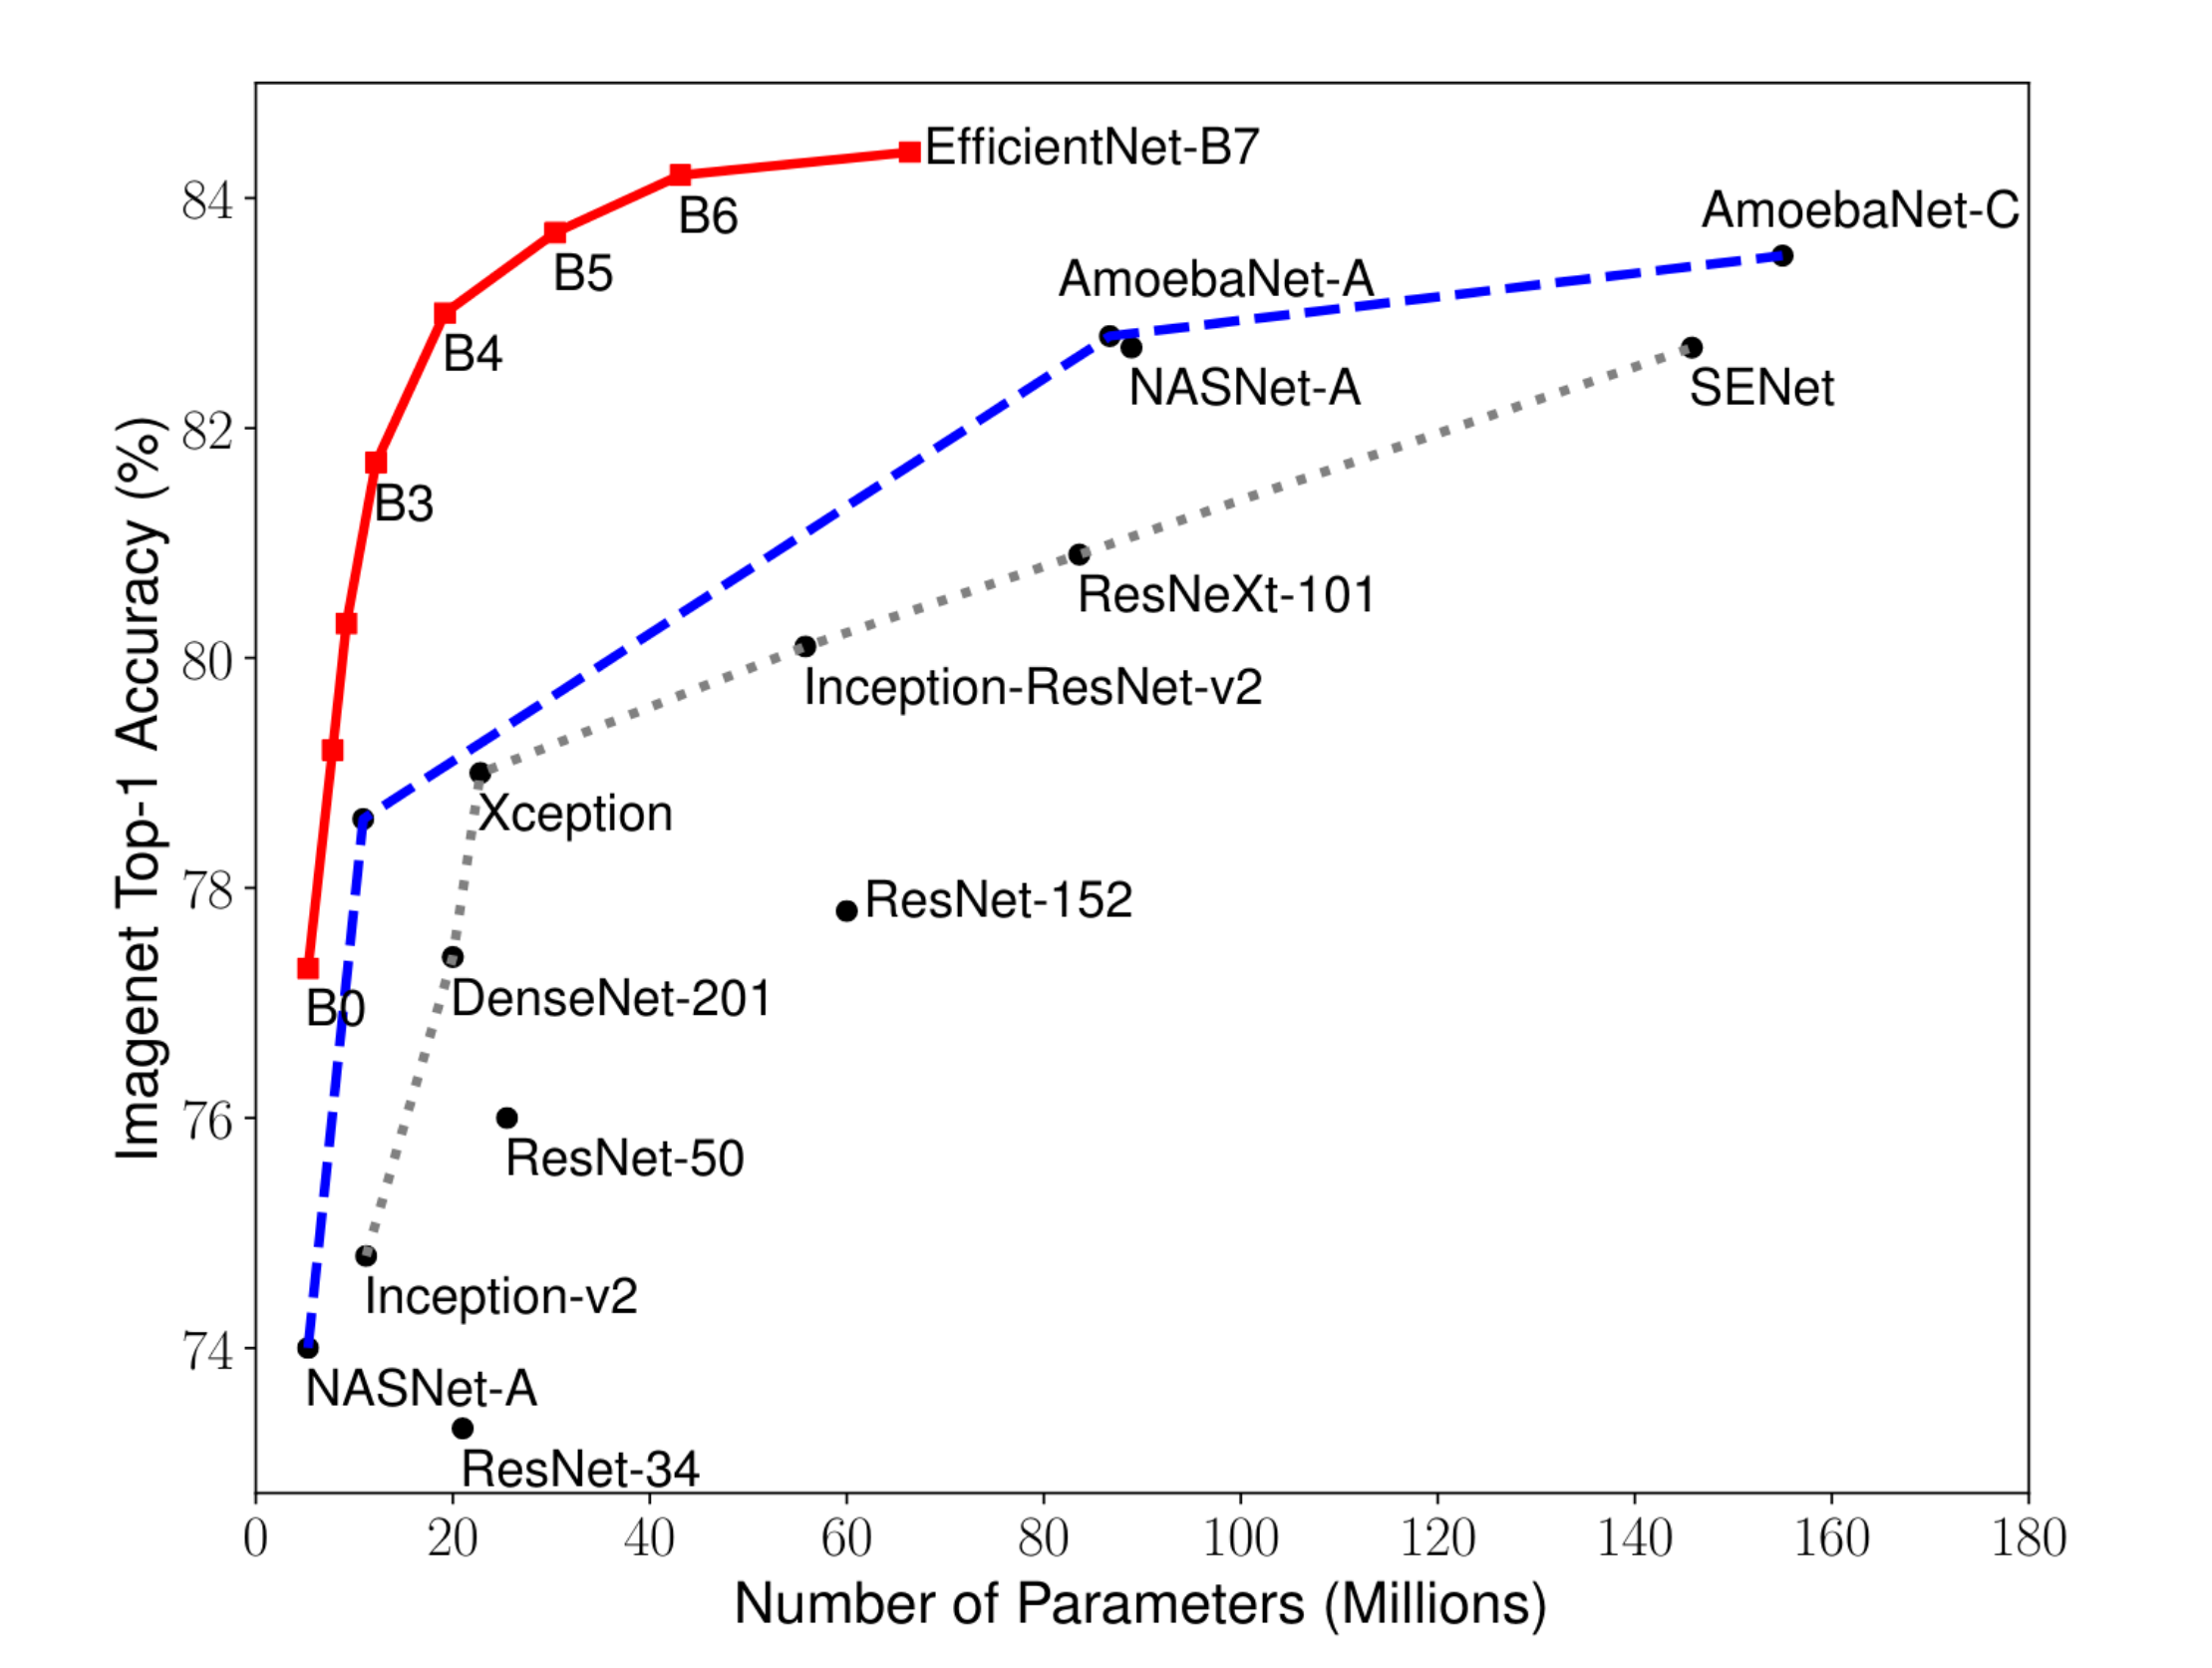
\includegraphics[width=0.8\textwidth]{imgs/imagenet_parameters.png}
\caption{Number of parameters in popular ImageNet classifiers. Figure from \citep{efficientNet}.\label{fig:params}}
\end{figure}

Picking which classifier to use as a base is often problem-dependent. As it is not possible to declare one network structure to be the best at all tasks, picking the best model to start with usually requires the user to compare different architectures and weighing the requirements for the problem at hand. Often though, the larger models will perform better, and there exists a correlation between performing well on ImageNet and being a good transfer learning model \citep{betterTransfer}. Though as can be seen in figure 3.1, better performance often comes at the cost of many more parameters, requiring more memory to train the model. Though, as the results in \citep{classifierPerformance} show, just the number of parameters is not the only thing to compare as the throughput of a Resnet50 turns out to be about three times as large as the throughput of an EfficientNet-B4 \citep{efficientNet} even though they have a similar amount of parameters. So in the case of time-constrained inference environments, also the time required for an inference has to be taken into account when picking models.
Often though, the number of parameters is a relatively good proxy for the inference time.
The throughput is likely due to the differences in the internal implementations of the EfficientNet and normal CNNs.

If there is enough data, it turns out that using a pre-trained network does not provide any benefits in terms of the converged model accuracy, but it is not detrimental to performance either \citep{rethinkTransfer}. When training sufficiently long on a sufficient amount of data, the pre-trained and randomly initialized networks converged to similar accuracies but required significantly different amounts of training resources. Still, this does not mean that pre-training is useless by any means as the saved resources and getting models to converge faster are essential factors for progress. And of course, there is not enough data in many cases, and training from scratch will not provide satisfying results due to the large number of parameters that would need to be optimized.
In these cases, it would then be a decision to apply transfer learning or to get a model that is not good enough to produce reliable results.

\section{ResNet}
ResNet is one of the first effective and very deep Convolutional Neural Network architecture that was presented in 2015 and won the ImageNet challenge. Prior to the publication of ResNet, the most powerful networks were relatively shallow, like VGGNet \citep{VGG}, which has only 19 layers. One of the big issues relating to training deep networks is vanishing gradients, where gradients disappear when they are backpropagated through many layers \citep{wideResNet}. ResNets utilize residual connections around bottleneck building blocks, which allow for the networks to contain many more layers than those without them, the largest network presented in the original ResNet paper was 152 layers, totaling for around 8x increase in the number of layers when compared to earlier networks \citep{resNet}.

\begin{figure}[h!] 
\centering 
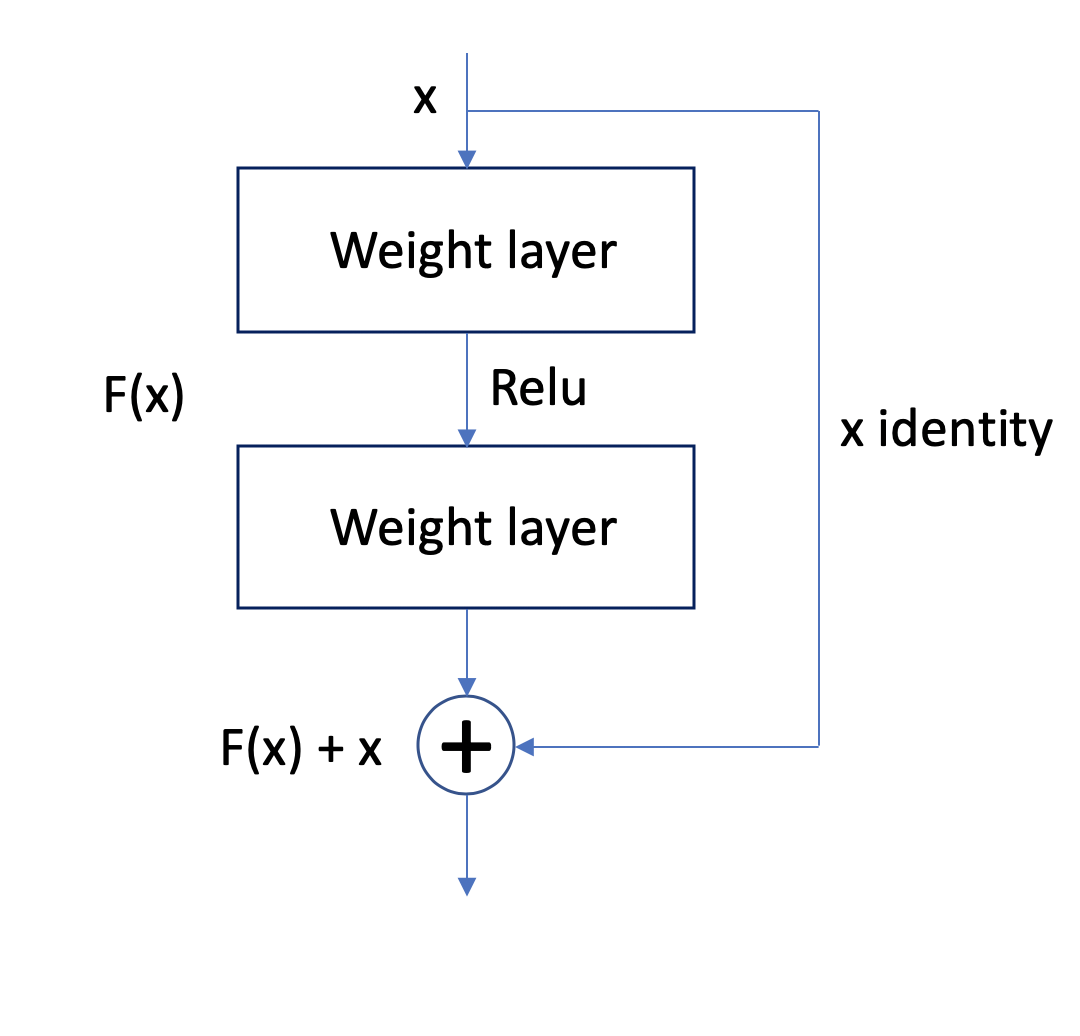
\includegraphics[width=0.8\textwidth]{imgs/resnet-block-own.png}
\caption{Resnet building block for learning the residual \citep{resNet}}
\end{figure}

The ResNet block architecture allows for the blocks to learn the identity function more efficiently by trying to learn the residual function instead of the direct mapping. The residual can be learned by adding the unchanged weights of an earlier layer to the output of some transformations on it.
The residual block is shown in Figure 3.2.
Normally a neural network layer learns the mapping between ${x}$ and ${y}$ using a function ${H(x)}$, but by the same token, we can learn a residual transformation.
Learning these residuals using the identity mapping skip-connections is the revolutionary idea introduced by the ResNet.
Since these residual connections are only connections, they do not require extra parameters to be learned and are free in terms of learnable parameters.
The residual transformation is
\[{F(x) = H(x) - x}\] \noindent where ${H}$ is the mapping of two or more network layers. Both of these approaches should approximate the same functions; the difference is in how easy it is for the network to learn. Learning a transformation of ${F(x) = 0}$ would intuitively seem easier for a neural network than learning ${F(x) = x}$. As can be seen from the success of the ResNets compared to non-residual networks, this is what allows for creating very deep networks. If the transformation changes the input size, a matrix ${W}$ is necessary to map the input to the same dimensions, generating the final formula for a residual block. \[y = F(x, \{W_i\}) + W_s x\] \noindent where $W_i$ and $W_s$ are the the weight matrices to be applied to x.

Many variants of ResNet exists, such as wide ResNets \citep{wideResNet}, ResNeXt \citep{resNext} and others. Also the DenseNet \citep{denseNet} is heavily inspired by ResNets. ResNet-50, ResNet-34, ResNet-101, and ResNet-152 are still some of the most popular models to use when a pre-trained ImageNet trained backbone is needed for some part of a classifier as they produce good results and do not contain too many parameters compared to some other architectures.

\section{Improving model performance}
Improving model performance is not easy, but using the various types of skip-connections, such as the ones used in ResNet residual blocks with the identity transform, it is possible to increase the size of the network to massive sizes. A 557 million parameter model called GPipe \citep{gPipe} takes the model scaling to the extreme and requires some unique parallelism libraries to train the model. It is still only slightly better than previous models, showing that size is not the only thing that matters.

\begin{figure}[h!] 
\centering 
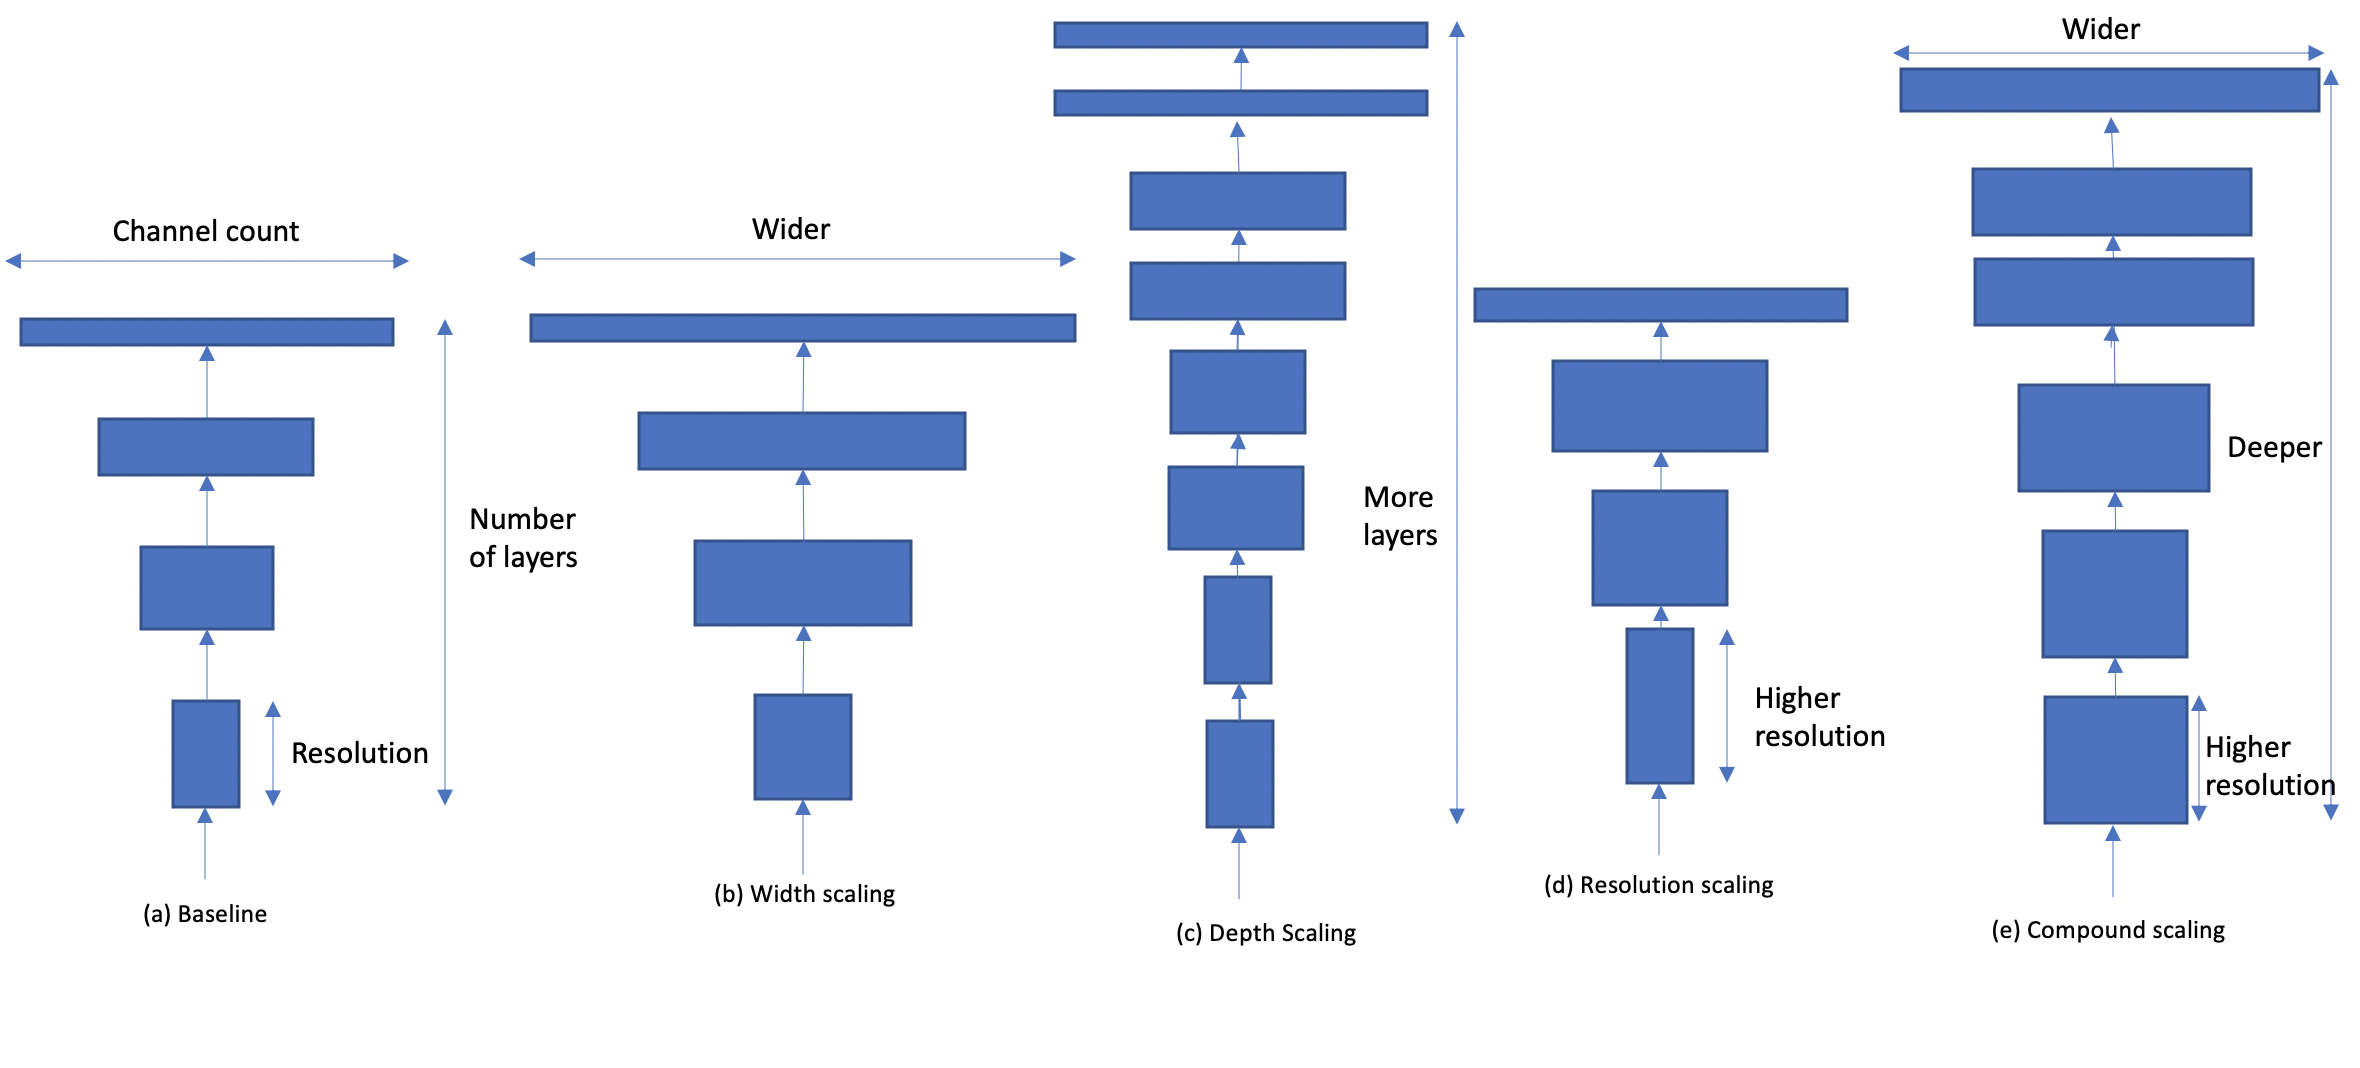
\includegraphics[width=0.8\textwidth]{imgs/scaling-networks-own.png}
\caption{Various ways of scaling network architectures \citep{efficientNet}. a) Shows the baseline network. b) Shows how to scale by the number of channels. c) Shows how to scale the number of layers. d) Shows how to scale by resolution. e) Shows how to scale all the metrics with a compound factor.}
\end{figure}

There are three main ways to scale up a network, as shown in figure 3.3. Scaling by depth means adding more layers to the model, allowing for more complex dependencies to be captured by the model. For example, ResNet-1000 is a very deep type of ResNet, but it has similar performance to a ResNet-101, so there are diminishing returns when trying to scale up by depth \citep{efficientNet}. Scaling by width means increasing the number of channels in the layers, and it is especially popular when optimizing smaller size models, such as MobileNet \citep{mobileNet}. Wide ResNets \citep{wideResNet} increase the width of the ResNet blocks and allow for better features and easier training. The third way is to increase the resolution of the input. A higher resolution allows for the network to find more specific features as the level of detail increases, and often specific network architectures work best at one particular resolution.

The other approach to finding a better architecture is to use different kinds of blocks that are better. One way of finding better building blocks is by manual experimentation. The other, like in the case of MnasNet \citep{mnas}, is to pose the problem as an optimization problem and to use Neural Architecture Search \citep{neuralSearch} to find the optimal solution. In the case of MnasNet, the goal is to maximize the model architecture m in \[ACC(m) \times [\frac{LAT(m)}{T}]^w \] \noindent where ${T}$ is the target, by searching in a constrained space. So the goal is to optimize the accuracy (ACC) of the model with a given latency (LAT) on a specific device. The search produces small but very efficient models when the target device is a mobile phone.

\section{EfficientNet}
EfficientNet models form a family of models ranging from EfficientNet0 to EfficientNet7 that were generated by smartly scaling existing convolutional models to optimize them for efficiency in a similar way to MnasNet \citep{efficientNet}. 
The more complex models are created by using compound scaling on the EfficientNet0 model, shown in Figure 3.3 (e),  where the width, depth, and the resolution of the network are scaled using a factor ${\phi}$. 
As the cost of neural architecture search grows exponentially as the size of the network grows, the search is only done on the base model. 
The search of ${\phi}$ is a constrained optimization problem, where width, depth and, resolution are constrained such that ${d^\phi \times w^\phi \times r^\phi \approx 2}$ and each increase in ${\phi}$ increases network FLOPS by ${2^\phi}$. 
The architecture search for the base network is similar to that of MnasNet. The target of EfficinetNet is to maximize the model m  \[ACC(m) \times [\frac{FLOPS(m)}{T}]^w\] \noindent so the goal is to optimize for both accuracy (ACC) and number of floating-point operations (FLOPS) instead of latency as in MnasNet \citep{efficientNet}. 

As seen in figure 3.1, these optimizations allow for the EfficientNet to form a very performant architecture using a low amount of parameters that does well on ImageNet and is good at Transfer Learning also. Interestingly though, the reduction in FLOPS and parameters do not directly translate to low real-world inference time. As is compared in the paper, an EfficientNet-B1 gets a 5.7x speedup over a ResNet-152, while the EfficientNet scores significantly higher on ImageNet. So in terms of the time and accuracy ratio, the EfficientNet seems to do well. When looking at the inference time in terms of FLOPS and parameters, we can find out that the ResNet would be more efficient, as the ResNet has 7.6x as many parameters and 16x FLOPS when compared to the EfficientNet, but the inference time multiplier is 5.7x. From this comparison, we can easily see that the number of FLOPS is not a direct proxy for inference time. 
Instead, the optimization should be for latency directly as in MnasNet if that is the goal.

The proposed EfficientNet models use mobile inverted bottleneck (MBConv) blocks used in MobileNetV2 \citep{mobileNetv2} in constructing the base model. The MobileNet uses a Depthwise Separable Convolution, where a depthwise convolution and a pointwise convolution are applied in sequence. The depthwise convolution applies ${d_i}$ ${k x k}$ filters to the input, where ${d_i}$ is the input channels and ${k}$ is the kernel size leading to an output channel count ${d_j = d_i}$. A normal convolutional layer would apply multiple filters having ${M}$ channels with the computational cost of ${h_i w_i d_i d_j k^2}$, whereas the depthwise convolution only has a cost of ${h_i w_i d_i (k^2 + d_j)}$, reducing the cost by ${k^2}$. The result of the depthwise convolution then runs through a pointwise convolution, where a ${1 \times 1 \times d_j}$ 1d convolution is applied to get the final output as a linear combination of the channels. The inverted residuals in MBConv are connections similar to ResNet, but in this case, they are connected between the low dimensional layers.

\section{Training image classifiers}
An image classifier's basic function is to predict which of some set of classes exists in an image.
So, to train a model to answer such a question, a data set with images and accompanying labels are needed.
For example, the Oxford-IIT Pets dataset \citep{catsdogs} consists of images of 37 different cat and dog species and labels for those images signifying which of the 37 classes an image represents.
The dataset consists of about 200 images per class, so it is relatively small and an excellent example of a situation where transfer learning is instrumental in getting good results.

After the data of the images and labels are gathered to a data loader, that outputs small batches for training, the model needs to be constructed.
For the backbone, any ImageNet classifier will do. 
For example, EfficientNet-B4 could be a good decision.
So we will initialize the backbone of our model with the weights of a pre-trained EfficientNet that was trained on the ImageNet data set by someone with access to large computational resources.
After the model has been initialized, the head has to be changed to be compatible with our new task.
By default, the model will be expecting to classify images to the thousand classes of the ImageNet.
In this case, we want to solve the 37 cat and dog species problem, so the final fully connected layer has to be changed.
It will be initialized as a fully connected layer with 37 output units, representing each of the classes, connecting the embedding to the outputs.
The head does not need to be just a single, fully connected layer, but it could also contain more fully connected layers, dropout layers, and batch normalization layers and more.
Adding more than a single fully connected layer might be a good idea if the backbone remains frozen and is not fine-tuned. 
That way, the head can learn some useful combinations of the image embedding instead of optimizing the features in the backbone.

Once all the layers are in place, the model needs to be optimized with a training loop.
Every iteration, a loss needs to be calculated for the batch that has been sampled from the data loader.
To be able to calculate the loss, the outputs of the final fully connected layer need to be normalized into a distribution of probabilities with softmax.
The softmax is defined as
\[{Softmax(x_i) = \frac{exp(x_i)}{\sum_j exp(x_j)}}\] \noindent
For each class $i$, there is an output score of $x_i$, for which we will calculate the proportion of its score with respect to the sum of all the classes' scores $x_j$, creating the probability distribution.
Since we have a single correct class, we would want to maximize the probability of the correct class and minimize the probability of the other classes.
The loss function to do exactly this optimization is called categorical cross-entropy, and it is defined as follows.
\[{CE = -\frac{1}{N}\sum_{i=1}^{N}(y_i * log(p_i) + ( 1 - y_i ) * log ( 1 - p_i))}\] \noindent
Where $N$ is the number of classes, $y_i$ is either 1 or 0 depending on if it is the correct label and $p_i$ is the probability for that class.
This formula does exactly what we previously described that we wanted to do.
To get the loss for a single class, if $y = 1$, the value will be the first part of the sum, if $y = 0$, the value will be the second part of the sum, since $(1 - y_i)$ is now 1.
When we optimize the model, in the case of the chosen architecture, the model will reach around 95\% accuracy on this data set \citep{efficientNet}.
\chapter{Multi-task learning}
Maybe drop some sections if it becomes too long.
\section{Definition}
Formally define multi-task learning similar to Transfer Learning using the original multi-task paper \citep{origMultitask}, and a newer view on the domain \citep{surveyOnMultiTask}.
\section{Benefits}
Inference time, regularization, smaller models etc. Weighing different tasks and getting information from the loss functions \citep{lossWeighting} \citep{usingUncertaintyToWeighLosses}
\section{Soft parameter sharing}
Define soft parameter sharing between tasks, show an example from \citep{mutualLearning}.
\section{Hard parameter sharing}
Show how multiple heads can be combined to produce outputs for various tasks using different heads, show results from sharing all/some layers. \citep{visualPerson} \citep{selfDriving} \citep{healthyDrink}
\section{Special multi-task learning techniques}
Show how an attention layer can be added to augment the performance in various tasks in a multi-task setting \citep{multiTaskAttention}. Also cross-stich networks \citep{crossStitch}.
\section{Multi-task learning with little data}
Why it can be beneficial with little data \citep{surveyOnMultiTask} Show some results where it is beneficial on little data.
\section{What and when to share}
Some ways to decide when multi-task learning might be a good idea and how to evaluate which tasks might be good to learn in a multi-task setting \citep{taskonomy} \citep{whichTasks}.
Show how this problem can be similar to deciding whether Transfer Learning is a good idea \citep{whatAndWhereToTransfer} \citep{transferringMidLevelRepresentations}
\chapter{Object detection}
Object detection is another prevalent task in the domain of computer vision.
An object detection task is one where the goal is to localize one or many different classes of objects using bounding boxes.
Before current deep learning-based techniques, a popular way to solve the problem was to use handcrafted features like in image classification and to use a sliding window over the image for localizing objects.
These previous techniques include, for example, the Viola-Jones detector \citep{viola-jones}, which uses a sliding window and AdaBoost for features, and another popular method was using histograms of oriented gradients \citep{hogs} to find where the boundaries of objects exist.
These days there exist various ways of using the feature maps of neural networks for learning the filters to get much better results.
The various architectures can be split into two approaches, one-stage detectors, and two-stage detectors.
The two-stage detectors require region proposals, based on which the object detection is done.
An often-used family of these kinds of methods is the R-CNN classifiers, for example, the faster R-CNN \citep{faster-rcnn}.
In the one-stage detectors, features from various layers of the classifier are used to get the predictions.
For example, the YOLOv4 \citep{yolov4} is the 4th iteration of the single-stage YOLO family of detectors that are very popular due to the good balance between fast speed and good accuracy.

\begin{figure}[h!]
    \centering
    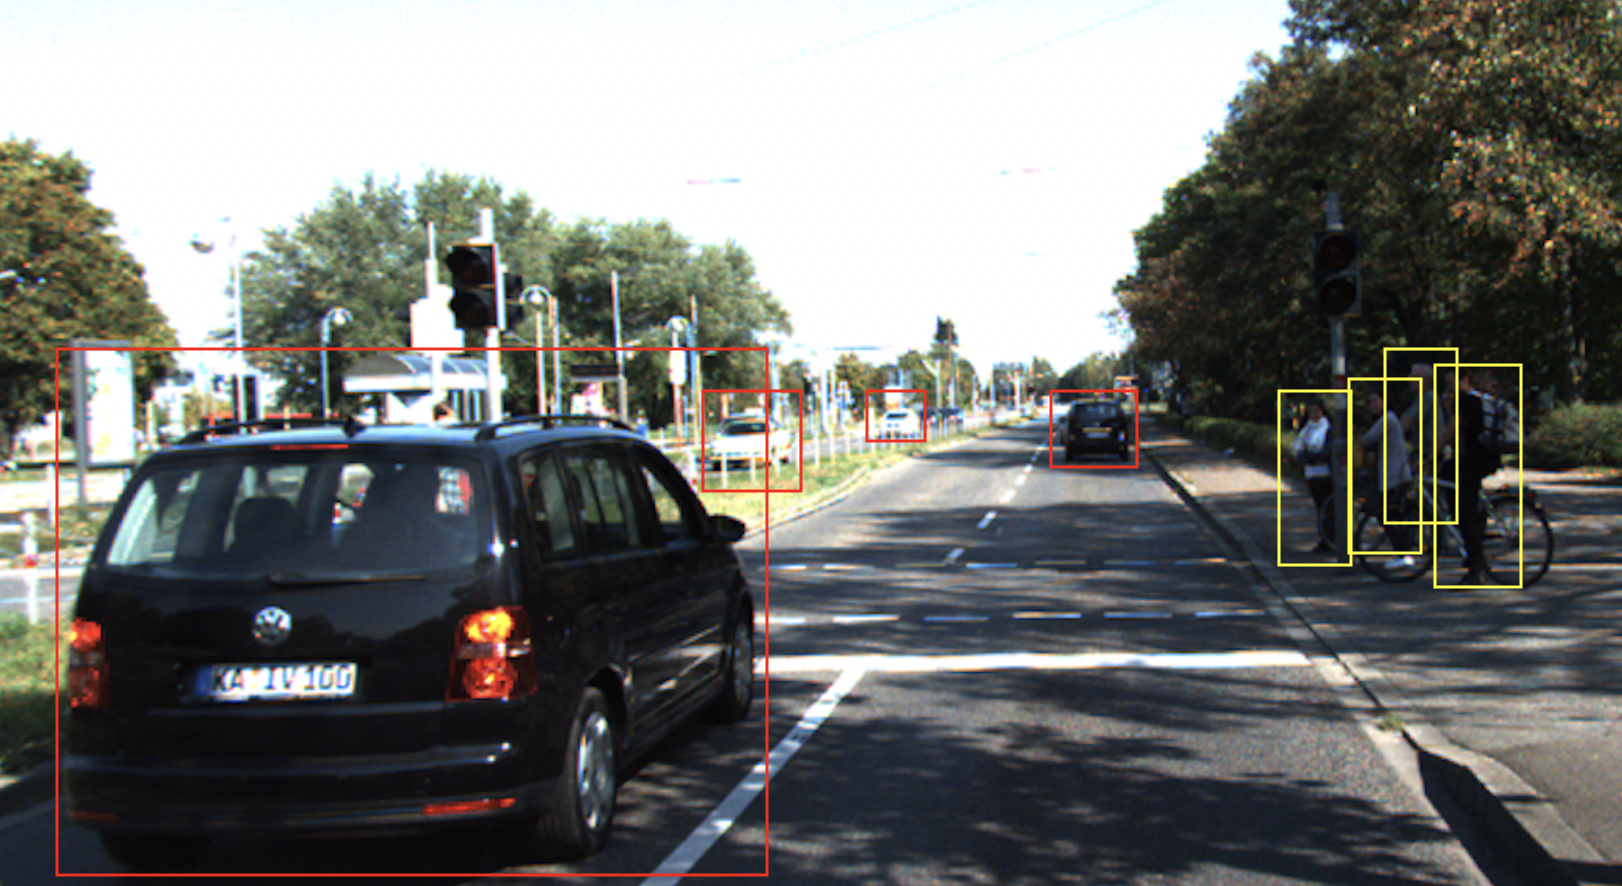
\includegraphics[width=0.8\textwidth]{imgs/obj-det.png}
    \caption{Object detection image labeled for people and cars.}
\end{figure}

\section{Metrics}
The training of object detection models requires data sets that have been labeled for that purpose.
Generally, the data sets contain bounding box annotations for each of the classes in the data set, such as seen in Figure 5.1.
For this reason, object detection models can't use a simple metric like the basic accuracy in image classification.
As the images are often manually labeled, the boxes are most likely not completely consistent.
So most likely, the predictions are never going to align with the labeled boxes perfectly.
Consequently, the method for evaluating object detection performance is Average Precision (AP) or mean Average Precision (mAP) or one of their variants.
These metrics use intersection over union (IoU) score to evaluate how incorrect the predicted bounding box is when compared to the actual label. Intersection over union is visualized in Figure 5.2.

\begin{figure}[h!]
    \centering
    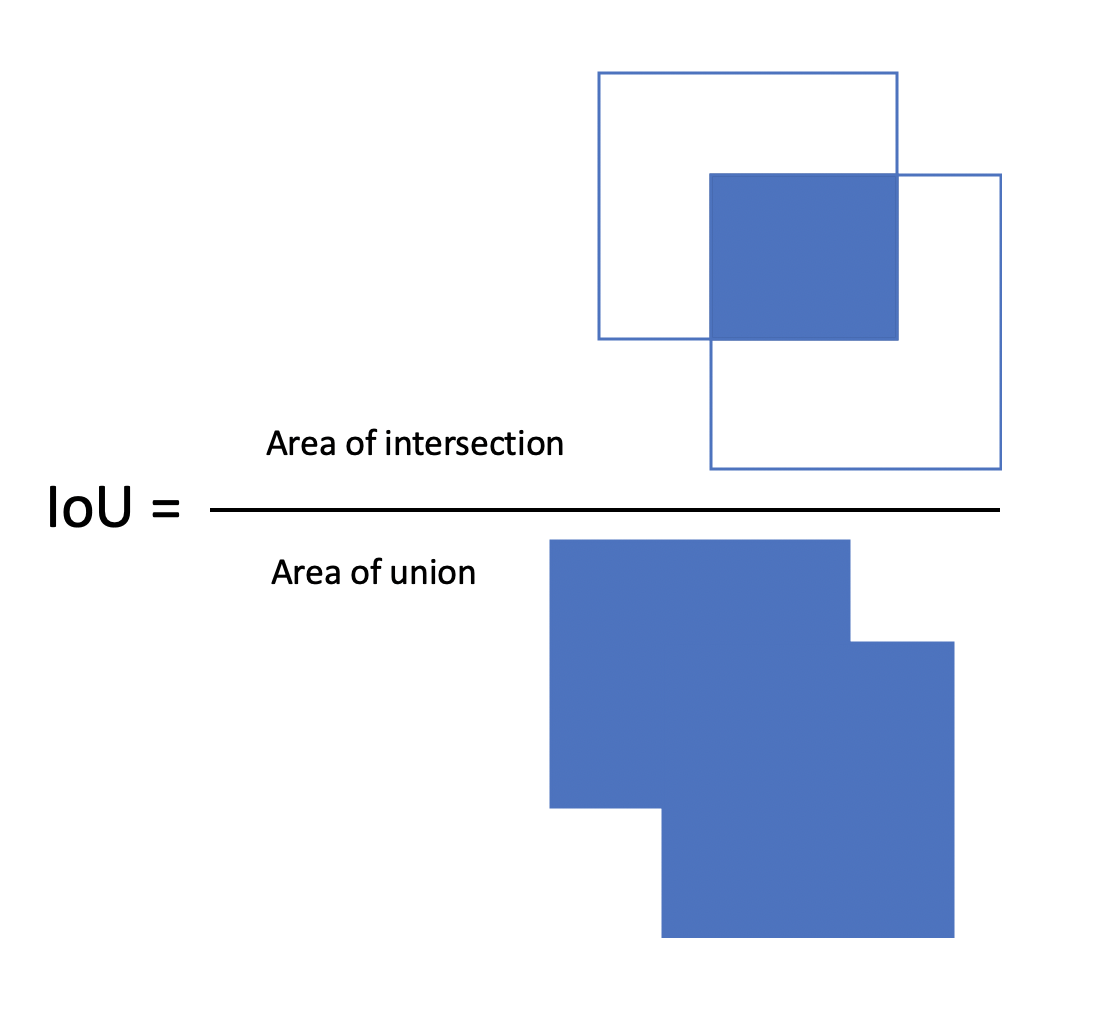
\includegraphics[width=0.8\textwidth]{imgs/IoU-own.png}
    \caption{The visual formula for calculating intersection over union.}
\end{figure}

To get to a final AP score, the first thing that has to be decided is the IoU score threshold for considering a prediction to be correct.
For example, we could consider all predictions that have over 50\% or 75\% overlap in the IoU.
The threshold value for IoU that should be used is not entirely standardized, and there are multiple ways of calculating the AP score.
For example, the popular COCO dataset \citep{COCO} uses an average of 10 IoU scores ranging from .5 to .95 IoU thresholds as the main metric.
To get the AP for a class, we need to graph the precision-recall curve and then calculate the area under it.
For example, the Pascal Visual Object Classes Challenge (VOC) \citep{PVOC} recommends doing this by using 11 points of interpolated precision.
So we get the following formula for Average Precision:

\[AP = \frac{1} {11} \sum_{r \in \{0, 0.1, \ldots, 0.9 , 1\}}{p_{interp}(r)}\] \noindent

Where $p_{interp}$ is defined as

\[p_{interp}(r) = \max \limits_{\tilde{r}:\tilde{r} \geq r} p(\tilde{r})\]

Then to get the mAP score, we can average the AP score for each of the classes in the data set.
As was mentioned, this way of calculating the AP is not always the same, for example, the COCO metrics \citep{COCO_SITE} recommend using 101 points for integrating the curve instead of the 11 proposed in the VOC.
This discrepancy in the integration means that not all AP scores are directly comparable.

\section{Object detection model structure}
Much like image classifiers and many other vision tasks, modern object detectors rely on pre-trained backbones to generate the features required for predicting bounding boxes.
A classifier head is required to get these predictions, but in object detectors, this head is more complicated than in image classification.

For the backbone, most object detection architectures use one of the same ImageNet models as in image classification such as ResNet or VGG.
However, the YOLO models use DarkNet, which is specifically designed for achieving efficient results in object detection \citep{yolov4}.
The main reason for picking one backbone over another is often a function of both accuracy and inference time.
As object detectors are often run on video data, inference time can be more significant than in image classification, as it is often desirable to be able to run them in real-time.

The head is where the architectures differ the most, and generally, any backbone could be combined with a specific detector head.
The head comprises of a neck, which connects the intermediate features from the backbone to the final head.
The intermediate features are generally connections from some specific layers of the backbone.
Earlier single-stage detectors used the extracted features directly, but the current state-of-the-art methods use special feature pyramids and path aggregation to get the best results \citep{efficientDet}.
For example, the YOLO v4 uses spatial pyramid pooling \citep{SPP} over the DarkNet features and path aggregation net (PANet) \citep{PANET} to concatenate the parameters for the classifier head \citep{yolov4}.
Different ways of combining the feature pyramids are described in Figure 5.3.
Like many other parts of the architecture, picking one is a trade-off of more parameters and inference time and accuracy.
\begin{figure}[h!]
    \centering
    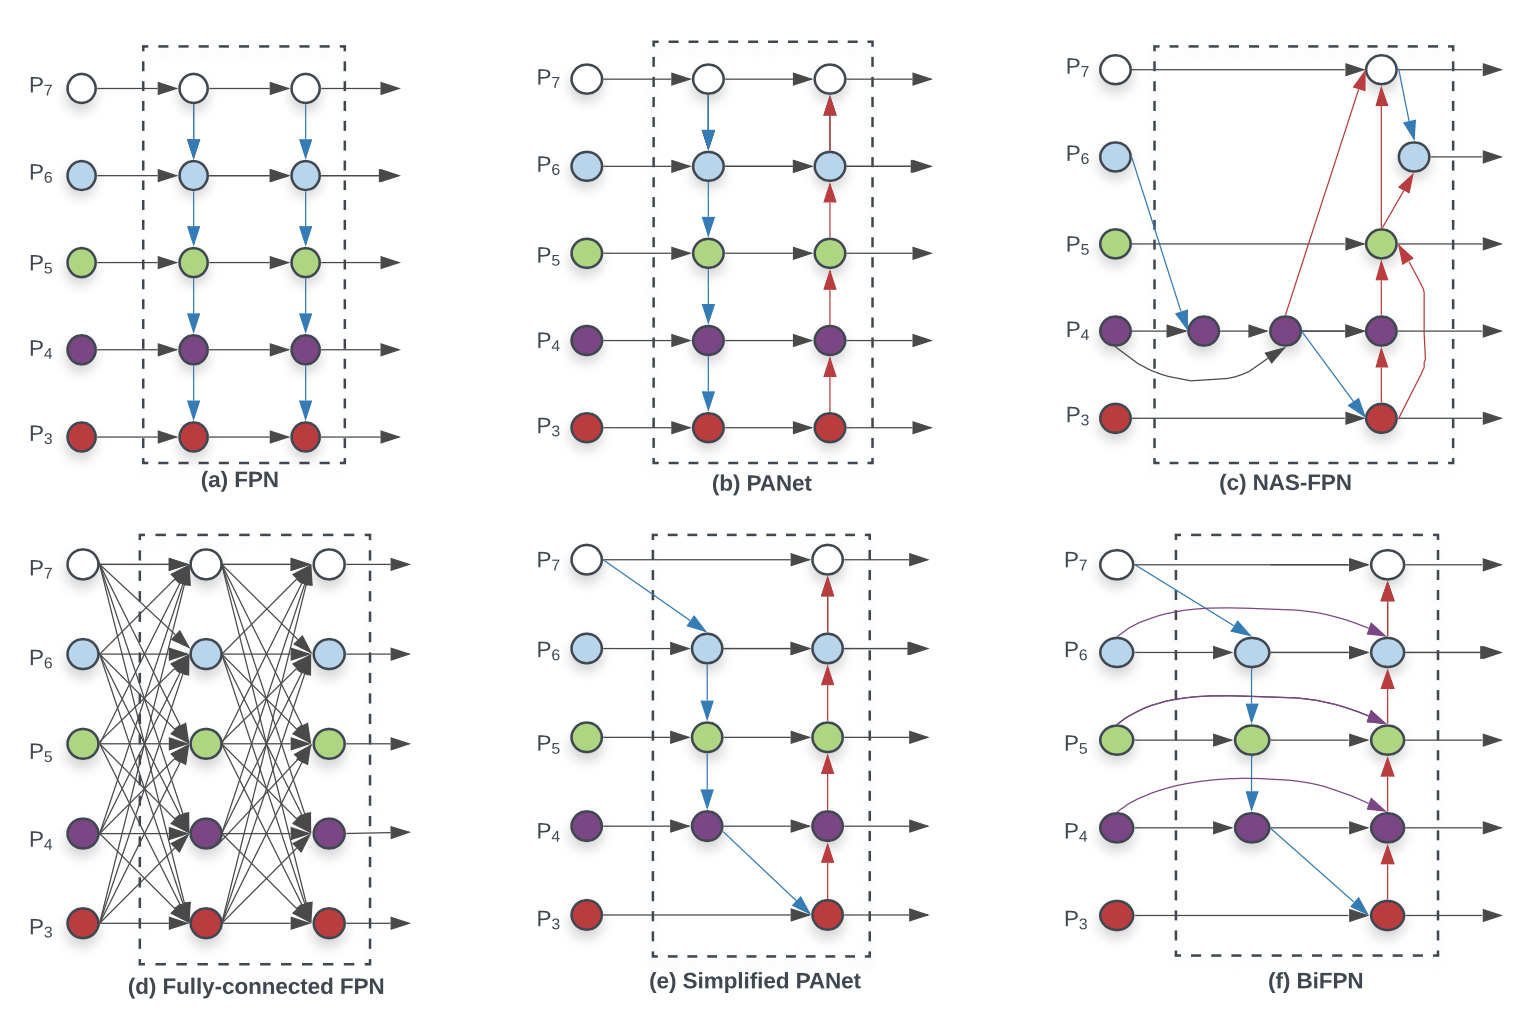
\includegraphics[width=0.8\textwidth]{imgs/detector_necks.png}
    \caption{a) Basic FPN \citep{FPN} where features are combined in only one direction. b) PANet modifies the basic FPN by adding a path from the lower level features to higher-level features. f) BiFPN tries to prune the connections to the most important ones. Image adapted from \citep{efficientDet}.}
\end{figure}

In two-stage detectors like faster R-CNN \citep{faster-rcnn}, there is a region proposal network (RPN), which predicts region proposals using a sliding window for some anchor boxes.
Running this RPN is expensive, and often the two-stage models are much slower than the single-stage detectors.
The benefit of the two-stage approach is generally a better accuracy. 
Still, recently the one-stage methods like YOLO v4 have achieved very similar accuracies to the two-stage ones with much faster inference times \citep{yolov4}.
By utilizing new ways of using the feature maps, the object detectors have recently become significantly better over the years, as can be seen from the different iterations of the YOLO models, as they have been using very similar backbones over the years \citep{yolov4}.

\section{Multi-dataset training}
Often an object detection problem requires detecting multiple different classes in a similar context.
For example, a self-driving car would need to detect various traffic signs, cars, pedestrians, road markings, cyclists, and many other things.
Collecting a single dataset that has labels for all of the classes of interest can be a very daunting task.
Even if it is feasible to create the dataset for the original classes of interest, this approach does not scale very well when new classes need to be recognized.
As likely the original dataset might contain millions of images labeled for multiple classes, adding a new class would require going through the entire dataset again and labeling the new class as well.
The new class may be relatively rare; for example, we may be interested in detecting emergency vehicles with sirens on.
Here is where multi-dataset learning is highly beneficial as it only allows for collecting a specific class dataset.
This type of cross-dataset learning is useful when we need to combine multiple distinct data sources to detect some union of the labels \citep{cross_data}.

The main difficulty in combining multiple datasets for detection lies in the fact that they likely contain unlabeled overlapping classes.
For example, given a dataset for detecting cars and another for detecting stop signs, we have two distinct datasets where only one of the classes is labeled.
If we train this model, assuming that the labels are genuinely valid, we will end up unlearning the tasks due to the overlap of the classes.
The problem lies in the fact that it is most likely that in the car dataset, we will find stop signs that are not labeled.
Similarily we will find cars that are unlabeled within the stop sign dataset.
When we naively train this model, we will end up detecting cars and stop signs that are actually correct but incorrect based on the labels.
The model will be punished for detecting these non-labeled positive examples due to the absence of the labels.

One way to do this is by disallowing the labels from incorrect datasets affecting the total loss.
For example, in \citep{cross_data}, the RetinaNet \citep{retinaNet} model's loss function is modified to ignore the losses for tasks that are not a part of the dataset.
All models using the same focal loss as RetinaNet can be trained with this adjusted loss function.
This way, each class will get its own positive and negative dataset to train on and not affect the performance of the other classes.
Still, this does not completely solve the problem as some of the classes might require conflicting features, as can be the case when very different tasks are combined. 
In that case, it could be smart to split the similar classes into different detectors and maybe share only the lower levels between all tasks.

Similar multi-dataset training can also be applied in multi-label image classification settings.
A multi-label image classification problem is one where we want to assign multiple labels to an image.
For example, we might want to classify whether it is raining, the sun is shining, the sea is visible, is there a dog in the image, and so on for all the classes of interest.
Again, collecting a dataset containing all labels for all images is quite expensive, but we can train this with a separate binary classification head for each task.
And as collecting a separate dataset for each task is relatively easy, it is possible to create a quite powerful model with relative ease.

\section{EfficientDet}
EfficientDet \citep{efficientDet} is an object detection model, that is based on the previously covered EfficientNet ImageNet model.
The neck for the EfficientDet is a unique bidirectional feature pyramid network (BiFPN).
The EfficientDet model also uses similar compound scaling as the EfficientNet models for the new object detection specific parts.
The scaling factor is used for the BiFPN network, box and class predictor networks, and to find the optimal input resolution.
The EfficinetDet shows that improving the backbone is quite useful for the entirety of the model.
This can especially be seen when looking at the comparisons of using a ResNet vs an EfficientNet as the backbone in the same EfficientDet architecture \citep{efficientDet}.
The EfficientDet model architecture is shown in Figure 5.4.

\begin{figure}[h!]
    \centering
    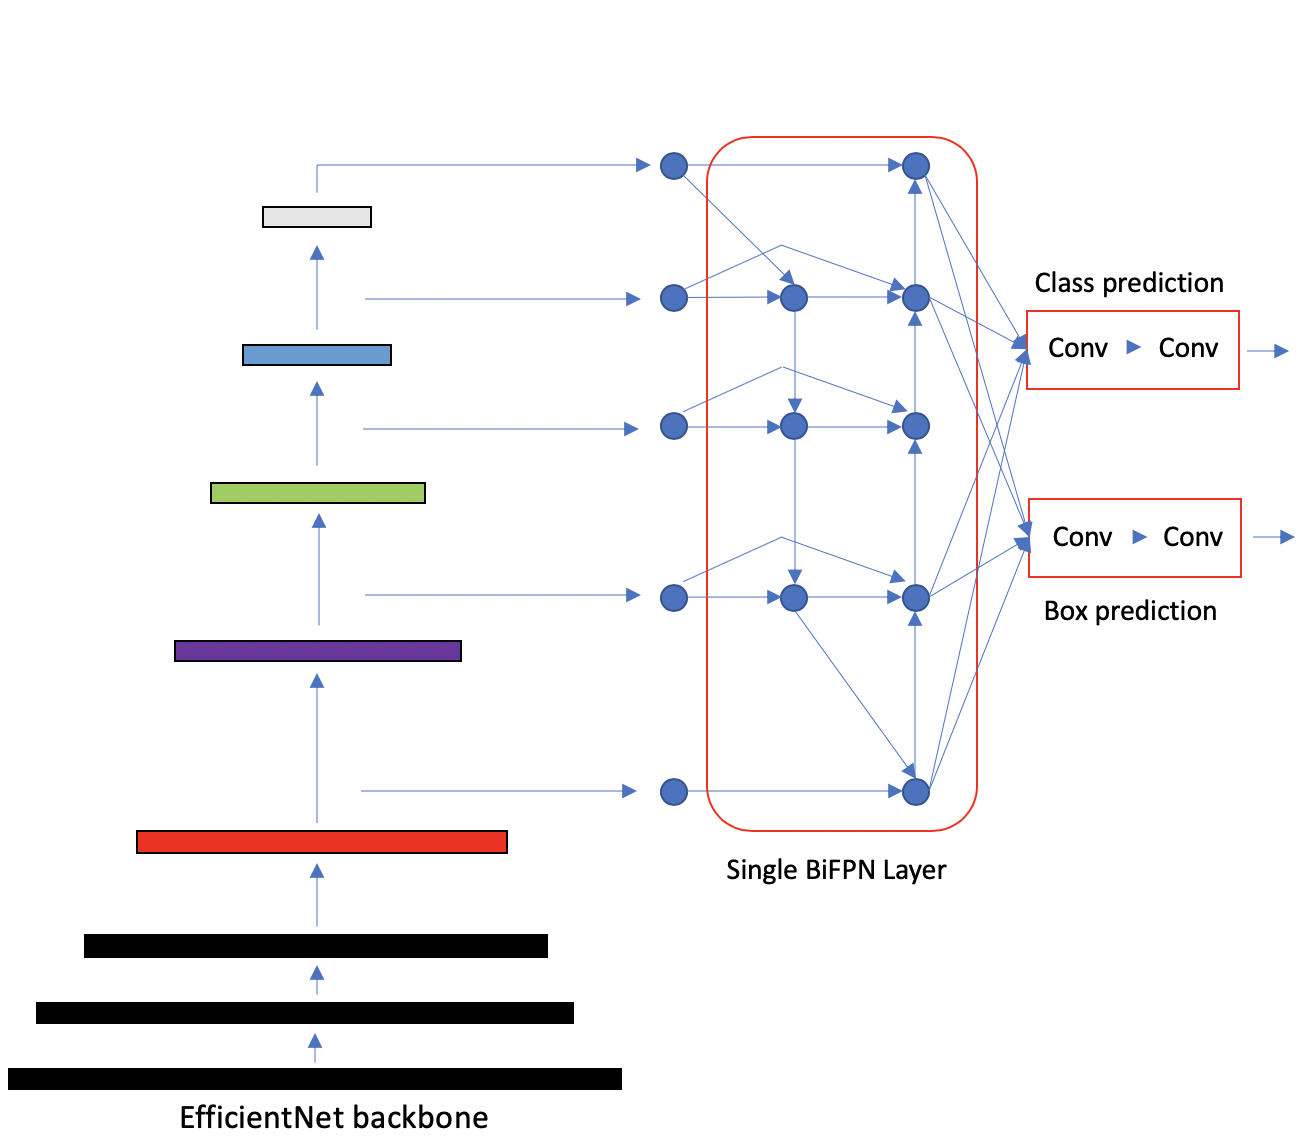
\includegraphics[width=0.8\textwidth]{imgs/eDet-own.png}
    \caption{EfficientDet architecture comprises of the EfficientNet \citep{efficientNet} backbone, the bidirectional feature pyramid network neck and the class and box classifier heads. Here only one BiFPN layer is pictured, but there are multiple of them normally stacked in succession.}
\end{figure}

The different feature maps in the BiFPN are combined using a weighted feature fusion.
The feature maps can't be directly combined since they have different dimensionality, so they have to be up or downsampled depending on the direction of the connection.
By weighing each feature map, the network can learn how important each feature map is.
Since the dimensionalities differ from one another, they likely don't contribute equally to the output feature maps, which is signified by the learned weight.
The BiFPN connection architecture is a simplified version of the PANet, as shown in Figure 5.3.
The goal of the changes from PANet is to have a more high-level fusion of features while dropping the nodes that have little feature fusion and then to stack multiple of these layers to get the final model \citep{efficientDet}.

The efficient scaling of the parameters and the BiFPN architecture allow EfficientDet to produce impressive results at relatively high framerates.
The new YOLO v4 produces very similar scores at acceptable framerates also \citep{yolov4}.
Still, some slightly better results are produced by the two-stage detectors, but those can't reach a 30 FPS inference time \citep{yolov4}.
So in practice, using either the EfficientNet or YOLO is a good idea when video needs to be classified.
The EfficientNet scales relatively well with larger EfficientNet backbones, but it is not possible to classify real-time video.
This flexibility allows for picking the model with a suitable accuracy for the problem at hand.

\section{Training object detectors}
As we described previously, object detectors are trained when there is a need to localize some set of classes within images by describing them with bounding boxes.
One widely used format for labeling such a dataset is the format for the object detection data in the COCO data set.
The COCO data consists of a set of images and a separate JSON file containing the labels.
The label file contains a list of all the images for the data set and a unique identifier for each image.
There is also an annotation list that contains a list of objects that specify the bounding box annotations.
The annotations are specified as being linked to a single image by its image id and defining the bounding box annotation dimensions.
The bounding box annotations are formatted by providing the coordinates of the top-left corner of the annotations and then the width and height of the box, so it is a tuple of four numbers (x, y, width, height).
To train on new data sets, they should be formatted similarly to make the training as easy as possible.

Once the data set has been gathered and collected in a correct format for the object detection task, a model needs to be picked.
Here, the final inference model's requirements need to be evaluated to decide whether a single-stage or a two-stage detector should be used.
For example, when running the model in real-time, a single-stage detector might be better, and in the case of doing text detection, it seems to be more popular to use a two-stage detector.
We will describe here how things work for the EfficientDet, which is a single-stage detector.

Once the exact architecture has been chosen, an implementation of it is needed to construct the model.
Generally, all the popular architectures have open-source implementations on GitHub in both Tensorflow and Pytorch, which are the most popular deep learning frameworks, that can be used.
Most of these implementations come quite readily wrapped in a way that given a correctly formatted data set, the models will be automatically initialized with the correct number of classes, and the training process is already specified by the input of a few necessary parameters.
As mentioned in the case of image classification, it is extremely important to initialize with the pre-trained weights with an object detection model to achieve the best results instead of training from scratch.
In an object detector, the problem-specific part is the number of classes in the classification head, which can be seen in Figure 5.4.
For the rest of the network, pre-trained weights should be used.

Training the EfficientNet itself is a multi-task training problem. 
We have two losses, the regression loss signifying how close the bounding boxes are to the annotations by calculating IoU and classification loss, which tells how incorrect the predicted labels are.
A major problem in optimizing anchor-based single-stage detectors like the EfficientDet is the fact that between the background no-class and the foreground classes of interest, there is a massive discrepancy in the number of instances to classify \citep{retinaNet}.
The anchor-based detectors determine whether an anchor placed at any valid spot in the image contains a class of interest or the background. 
There are tens of thousands to hundreds of thousands of valid anchors to consider depending on the architecture. 
Due to this, we can have a class imbalance of 1:1000 between the positive and negative cases.
For this reason, the recent single-stage detectors use a focal loss presented in the RetinaNet paper, to account for this class imbalance \citep{retinaNet}.

The focal loss introduces two new parameters to the cross-entropy formula to account for the class imbalance. 
The formula for focal loss (FL) is as follows.
\[FL(p_i) = -\alpha_i * log(1-p_i)^\gamma * log(p_i)\] \noindent
Where $\alpha$ and $\gamma$ are the new scaling factors and $p_i$ is defined as $p$ if y = 1 and $1 - p$ otherwise.
The factor $\alpha$ is there to weight the loss for the positive and negative cases separately. 
It is a parameter that is recommended to be set at the inverse class frequency, but the value can be searched by experimentation as well \citep{retinaNet}.
The factor $\gamma$ makes sure that a large number of easy classifications do not dominate the total loss.
For $\gamma$ the recommended value is two \citep{retinaNet}.
With this loss function, it is possible to have a very large number of anchors, where a large majority of them are always predicted as the background class.

With these, the object detection model can be trained.
Still, just leaving all the extra parameters at the default values may not produce the best results.
For example, the possible anchors that the model uses are specified using specific parameters.
The parameters that can be modified are the anchor size, depending on whether large or small objects need to be detected, the anchor sizes can be modified to suit the task at hand.
The anchors also have aspect ratios applied to them, which can be modified, the default ratios are 1:1, 2:1, and 1:2. 

\begin{figure}[h!]
    \centering
    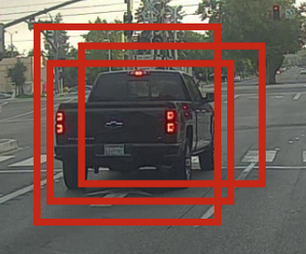
\includegraphics[width=0.8\textwidth]{imgs/nms.png}
    \caption{Object detection without non-max suppression. The same car is detected multiple times.}
\end{figure}

Finally, once a model has been trained with a suitable dataset, architecture, and hyperparameters, it can output predictions for new images.
If the model is used without any modifications, the output boxes will likely look like the predictions in Figure 5.5.
To fix this issue in the predictions, non-max suppression (NMS) should be used \citep{nms}.
With non-max suppression, we can achieve only a single bounding box that better represents what is most likely wanted.
In some cases, using NMS can lead to not being able to predict heavily overlapping classes.
Generally, though NMS should pretty much always be used to avoid the issue depicted in the Figure 5.5.

The object detectors are a good example of multi-task learning and how using the same feature maps, it is possible to solve multiple problems.
In this case, only a single annotation is needed to label for the two different tasks that can be optimized together.
Since we have two losses that are calculated, we can decide to focus on one of the losses by adding a multiplier to it and see if the higher loss could improve that task.
While some of the things covered here will be similar in the two-stage detectors, the region proposal network approach is very different from the anchor-based single-stage detectors covered in this section.

\chapter{Experiments}
As we have covered, the effect of a Multi-Task problem setting is challenging to quantify theoretically without experiments. 
Here we will take various datasets for object recognition, object detection, and pose estimation and see what the effects of training them in a multi-task setting are. 
The metrics we are mainly interested in are the reduction in model size, inference time, and model accuracy on the different tasks compared to the single-task counterparts.
We will also address the difficulty of the multi-task training process when compared to the single-task problem.
These issues will include trying different sharing architectures and searching for the new hyperparameters that provide the best possible results.
The experiments will focus on utilizing the previously presented EfficientNet and ResNet in various multi-task experiments to see how they compare.
The actual models will be EfficientNet-B3 and ResNet-101 since they require a roughly equivalent amount of memory to train.

\section{Training setup}
All the experiments use the same computer, and the model training is done using an Nvidia GeForce RTX 2070 GPU that has 8 GB of GDDR6 VRAM \citep{nvidiaRTX}. 
Thus all the models will have to be small enough to train on this relatively small amount of memory. 
The deep learning framework that is used to implement the models in all the experiments will be PyTorch \citep{pytorch} that is used inside Docker \citep{docker} containers. 
Also, Nvidia Apex \citep{Apex} will be used to train models using mixed precision floating-point numbers to reduce the size of the models and to increase the speed of floating-point operations. 
The model weights will be 16-bit floating-point numbers where it is safe to use the lower precision representation.
Besides the performance improvement, using lower precision floating-points can act as a regularizer as the model can't overfit on the high precision values and thus improve model accuracy as well \citep{mixedTraining}.

As a default for each task, we will use the following default procedures unless otherwise stated. 
For the Multi-task training process, we will sample the data sets for each task with a probability respective to its size. 
The loss function for every task has the same weight multiplier of one.
The batch size for each task will be maximized to fit within the memory requirement, giving a batch size of 32.
For weight optimizer, we will use SGD with a cyclic learning rate scheduler \citep{cycliclr}.

\section{Training loop}
The base training loop for a multi-task training problem is relatively similar to that of a single-task model.
Algorithm 1 shows the alterations that are needed for the training loop.
The main difference is that instead of a single data loader, batch size, and loss function, there needs to be one of each for each task that is trained.
Besides these, some values for the sampling ratios and possibly some values for loss weights are needed.
The loss weights can be omitted if there is no need to diverge from having a constant 1 factor for each of the losses.
One completely new part of the loop is the sampling of the task according to the ratios provided.
All the parts of the standard training loop can be chosen from the provided lists of parameters, and the training is as in a single-task model.

\begin{figure}[ht]
    \centering
    \begin{minipage}{.95\linewidth}
        \begin{algorithm}[H]
            \caption{Basic multi-task training loop}
            \KwIn{Epochs $e$, Data loaders $data\_loaders$, Sample probabilities $\alpha$, Batch sizes $B$, Training sets $X$, Model $model$, Loss functions $loss\_funcs$, Loss weights $w$}
            $batches \leftarrow \sum_i{ \dfrac{|X_i| \alpha_i}{B_i}}$

            \For{$epoch \in \{1,\dots,e\}$} {
                \For{$i \in \{1,\dots,batches\}$}
                {

                    {task\_id $\leftarrow$ sample($\alpha$)}

                        {(x, y) $\leftarrow$ next(data\_loaders[task\_id])}

                        {y\_hat $\leftarrow$ {model(x, task\_id)}}

                        {loss $\leftarrow$ loss\_funcs[task\_id](y, y\_hat) $\times$ $w[task\_id]$}

                        {loss.backward()}
                }
            }
        \end{algorithm}
    \end{minipage}
\end{figure}

The provided algorithm assumes that at a time, we are interested only in the labels of a single task per image.
If there is a need to train multiple tasks from a single input, then the minor adjustment that is needed is to sum the losses of multiple tasks that are backpropagated.
Otherwise, the training loop remains the same, even if multiple tasks are optimized from a single batch.

\section{Basic multiple object classification tasks}
As we have previously covered, fine-tuning an ImageNet classifier often produces good results. 
Here we will take a pre-trained ImageNet backbone and learn multiple object classification tasks using the shared image embedding.
First, we will use two datasets that both contain images of healthy and unhealthy plants.

\begin{figure}[h!]
    \centering
    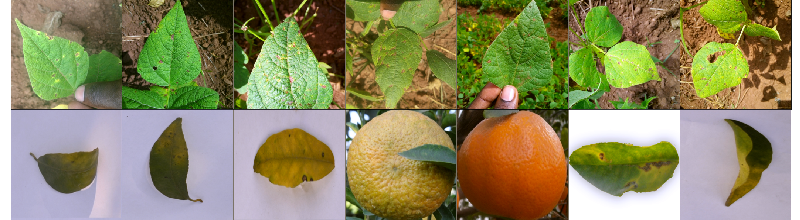
\includegraphics[width=0.8\textwidth]{imgs/citrus_beans_examples.png}
    \caption{Example images from the citrus and ibean data sets.
    The images in the top row are from ibean, and the bottom row is from the citrus data set.}
\end{figure}

The ibean dataset \citep{beansdata} contains 1296 images classified into three classes; Healthy, Angular Leaf Spot, and Bean Rust.
The data set provides a split for the images that will be the split that is used for the experiments.
The citrus leaves dataset \citep{citrusdata}, on the other hand, contains 759 examples of citrus fruits and leaves with six different classes; Black Spot, Canker, Greening, Scab, Melanose, and Healthy.
This set is quite tricky as it contains 609 images of leaves and only 150 images of actual citrus fruits, and some of the classes have very few images.
Some examples from the data sets are in Figure 7.1.
For the training split, the data will be split in 65/10/25 ratio for the training, validation, and test sets, respectively.
The goal of this kind of split is to have some relatively reliable test results by having proportionally larger than regular test set since there is so little data.
Both of these datasets have a relatively small amount of images available for training, so it should serve as a good basis for trying to train multi-task classifiers and give a glimpse into the adjustments that need to be made when training multi-task classifiers.
The goal for this experiment is to get familiar with the basics of how to create the multi-task models, and how to do the actual changes to the training loop in the Pytorch code to accommodate for the multi-task training.

When the two closely related datasets are used to train the model, we could expect the model to generalize better on both of them, as hopefully similar features would benefit both tasks.
But as the tasks are quite simple, the benefits can be relatively small as the likely accuracy for the single-task models should be quite high.
In the case of the citrus data set, learning to classify the citrus fruits could prove quite difficult, and for that, the bean leaves likely won't be of much help.
This model is depicted in figure 7.2.

\begin{figure}[h!] 
\centering 
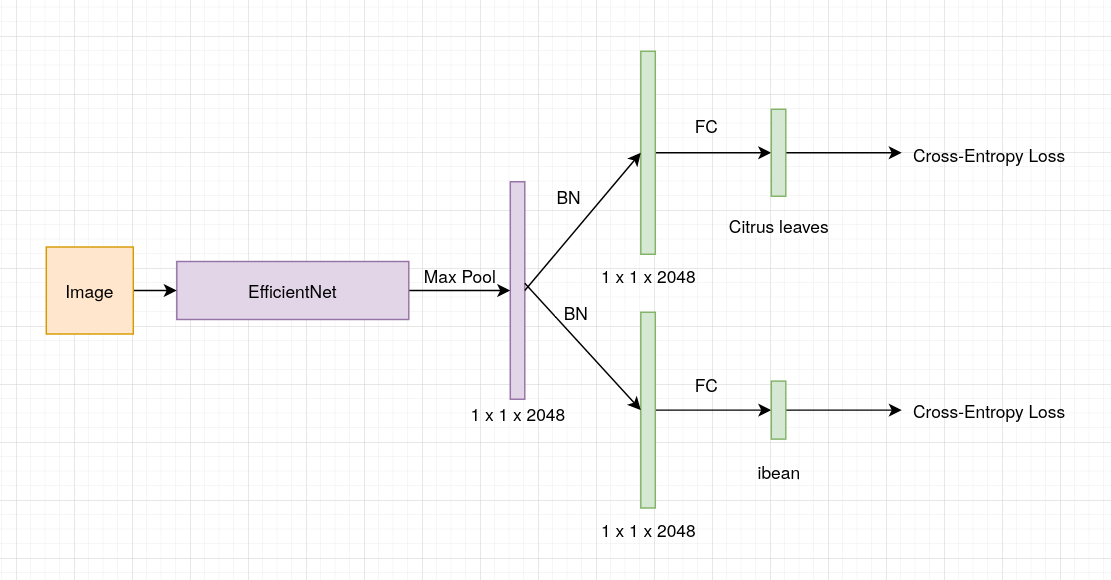
\includegraphics[width=0.8\textwidth]{imgs/object_classification_architecture.png}
\caption{Network architecture for two image classification tasks.}
\end{figure}

To further extend the generalizability, we will try to add a third somewhat similar classification task using the Oxford flowers102 dataset \citep{flowers102}, which contains 102 different types of flowers for classification. 
The assumption here would be that flowers could require similar features as the previous leaf classification tasks, thus when increasing the training data with a closely related task, we could increase the generalizability even further.

Multi-task and single-task models were created and evaluated for both EfficientNet and ResNet backbones.
For the single-task performance, in this case, the ResNet model did slightly better on both of the tasks achieving 96\% test accuracy on the beans dataset and 88\% test accuracy on the citrus dataset, and the EfficientNet model achieved 94\% and 84\% test accuracies on the tasks.
In terms of training, the most significant parameter is the sampling ratio of the two tasks.

The sampling was done with a random number to pick which data loader would be used for the current batch.
If the sampling is done by going through each of the datasets entirely one at a time, the model ends up at a point where only one of the tasks has good accuracy.
If the ratio is left as proportional to the data set size, the multi-task model ends up only learning to classify the ibean data set, and the accuracy for the citrus data will stay low.
After some experimentation, the suitable probabilities for achieving good results with the EfficientNet multi-task classifier were 0.66 for the citrus and 0.33 for the ibean data.
Interestingly, the same ratio does not directly transfer to the ResNet model. 
When we used the same ratio as with the EfficientNet, the model still seems to converge only on a good result for the ibean data set.
For the final results with the ResNet classifier, the sampling probability for the citrus dataset needed to be raised, and the value we ended up getting the best results with was 0.73.

\begin{table}[]
    \centering
    \begin{tabular}{lccl}
        \multicolumn{1}{l}{\textbf{}}    & \multicolumn{1}{l}{\textbf{ibeans}} & \multicolumn{1}{l}{\textbf{citrus}} & \multicolumn{1}{l}{\textbf{flowers}} \\ \cline{2-4}
        \textbf{Single-task models}      & \multicolumn{1}{l}{}                & \multicolumn{1}{l}{}                & \multicolumn{1}{c}{-}                \\ \hline
        \multicolumn{1}{l}{EfficientNet} & \multicolumn{1}{c}{94\%}            & \multicolumn{1}{c}{-}               & \multicolumn{1}{c}{-}                \\ \hline
        \multicolumn{1}{l}{EfficientNet} & \multicolumn{1}{c}{-}               & \multicolumn{1}{c}{84\%}            & \multicolumn{1}{c}{-}                \\ \hline
        \multicolumn{1}{l}{EfficientNet} & \multicolumn{1}{c}{-}               & \multicolumn{1}{c}{-}               & \multicolumn{1}{c}{97\%}             \\ \hline
        \multicolumn{1}{l}{ResNet}       & \multicolumn{1}{c}{96\%}            & \multicolumn{1}{c}{-}               & \multicolumn{1}{c}{-}                \\ \hline
        \multicolumn{1}{l}{ResNet}       & \multicolumn{1}{c}{-}               & \multicolumn{1}{c}{86\%}            & \multicolumn{1}{c}{-}                \\ \hline
        \multicolumn{1}{l}{ResNet}       & \multicolumn{1}{c}{-}               & \multicolumn{1}{c}{-}               & \multicolumn{1}{c}{97\%}             \\ \hline
        \textbf{Multi-task models}       & \multicolumn{1}{l}{}                & \multicolumn{1}{l}{}                & \multicolumn{1}{c}{-}                \\ \hline
        \multicolumn{1}{l}{EfficientNet} & \multicolumn{1}{c}{94\%}            & \multicolumn{1}{c}{88\%}            & \multicolumn{1}{c}{-}                \\ \hline
        \multicolumn{1}{l}{ResNet}       & \multicolumn{1}{c}{96\%}            & \multicolumn{1}{c}{89\%}            & \multicolumn{1}{c}{-}                \\ \hline
        \multicolumn{1}{l}{ResNet}       & \multicolumn{1}{c}{96\%}            & \multicolumn{1}{c}{91\%}            & \multicolumn{1}{c}{97\%}             \\ \hline
        \multicolumn{1}{l}{ResNet}       & \multicolumn{1}{c}{96\%}            & \multicolumn{1}{c}{-}               & \multicolumn{1}{c}{97\%}             \\ \hline
        \multicolumn{1}{l}{ResNet}       & \multicolumn{1}{c}{-}               & \multicolumn{1}{c}{85\%}            & \multicolumn{1}{c}{95\%}             \\ \hline
    \end{tabular}
    \caption{Accuracies on the data sets for both single-task and multi-task models with ResNet and EfficientNet.}
\end{table}

Training both tasks in a multi-task setting, we found that the accuracy on the citrus data set was increased, and ibean accuracy stayed the same.
Specifically, the accuracy for the EfficientNet classifier went up to 88\% and for ResNet up to 89\%.
The final model evaluated on the test set was the model with the highest average validation accuracy over the two tasks when trained for 25 epochs.
All the results are displayed in table 7.1.
The results show that even though these tasks were relatively simple and the accuracies for the single-task models were high, there was a benefit to be gained from multi-task training.
Here we mainly focused on getting good results on a fully shared backbone, and more experiments could be done by having fewer parameters shared between the tasks.
As an introduction to multi-task learning, the experiments show that picking the correct sampling ratio is extremely important for achieving desired results.
In that way, the sampling ratio seems quite unlike learning rate in that picking too small learning rate may lead to slow convergence but will most likely produce results in the end.
With the sampling ratio, it seems that the correct value needs to be found by experimentation, as a too low ratio for the citrus data gives accuracies that can be as low as 60\%.

Based on the results from the multi-task results on two tasks, we tried to add the third flower recognition task.
The flower recognition task has about 10 000 images and 102 classes, whereas the other two tasks have significantly less data and fewer classes.
On the two task experiment, it seemed that the sampling ratio should be relative to the task difficulty.
Here it would seem that the 102 class flower recognition should be much more difficult than the other two tasks, and we tried using sampling ratios in the range of about 0.5 to 0.7 for the flower task.
The best result achieved with these ratios was multiple percentage points below the single-task performance on all tasks.
However, when the flower task ratio was 0.1, it was possible to surpass the single-task results on all the tasks.
This training approach took significantly longer to converge to results.
The original sampling ratios converged in about five epochs to the best model, and the low flower ratio took about 50 epochs.
I started the training using the sampling ratio of 0.1 and decided to increase it up to 0.2 by the end of the training process.

When the training the model using the lower flower sampling ratio, it quickly converges close to the single-task performance on the two smaller tasks and slowly learns the flower task.
It is hard to say exactly why such low sampling ratios seemed to work.
Perhaps it has something to do with the difficulty of overfitting on a single task in a multi-task setting even though the small training set is seen so many times.
So the features for the smaller data sets are not just memorizing the pixels of the training set, but rather the features that generalize well.
Since the model already has good features for the smaller tasks and it is forced to find only a relatively minor shift in the parameters to learn the flower classification.
And seeing as the other tasks are improved as well, it shows that some of the features of the flower data are useful in the easier tasks.

From the three task models, the final model was picked as the one having the best average validation accuracy on all the tasks.
The final model wasn't just this model directly, though.
To get the final model, we froze all the shared weights and then did fine-tuning similar to what one might do when training a transfer learning classifier.
Having the model train on all the tasks using the frozen representations seemed to be useful.
The fine-tuning may be a good idea since, while training, the shared features are constantly shifting, and when one task is trained, it shifts the weights according to its gradients.
The other tasks won't have adjusted to the new, slightly shifted shared weights, which can lead to incorrect classifications.
When the shared weights are frozen, each of the task heads gets to learn the exact mapping from the shared representation to the outputs without them shifting during training.

All in all, these experiments validated the assumptions made about the multi-task training quite well.
Still, finding the sampling ratio is very laborious and not very intuitive.
This is why the results for the citrus and flower pair are worse since we spent less time finding the optimal ratios and mainly verified that it roughly works as expected.
Perhaps it could be automated to get somewhat decent indications of what should be tried.
The problem, in the end, is that even if some kind of grid search could be applied, it would take very long to predict the final metrics of the models, and as seen in the discrepancy of the flower ratios, it could take many epochs to get the final results.
Perhaps some kind of dynamic sampling ratio, where the task lowest relative to the expected accuracy is sampled more, could be beneficial.

\section{Multi-label classification}
For multi-label prediction, there can exist a problem where not all classes are restricted to only their data sets.
For example, a photo of a dog taken outdoors can contain other classes such as a person, sky, or sea.
These may not be labeled for that set but could be classes of interest.
If we train models on incorrect labels, it can lead to unlearning as the model may make correct predictions but is punished due to the absence of the labels for the images.
However, if the problem is posed as a multi-task binary classification problem over several classes, each task can have its own distinct data set with labels for only the single task.
Then upon training on an image containing other classes, there is no inverse learning as the image will not try to learn the other classes if there exists no certainty of that label.
Still, the problem is not gone as often any dataset has at least some mislabeled examples.

\begin{figure}[h!] 
\centering 
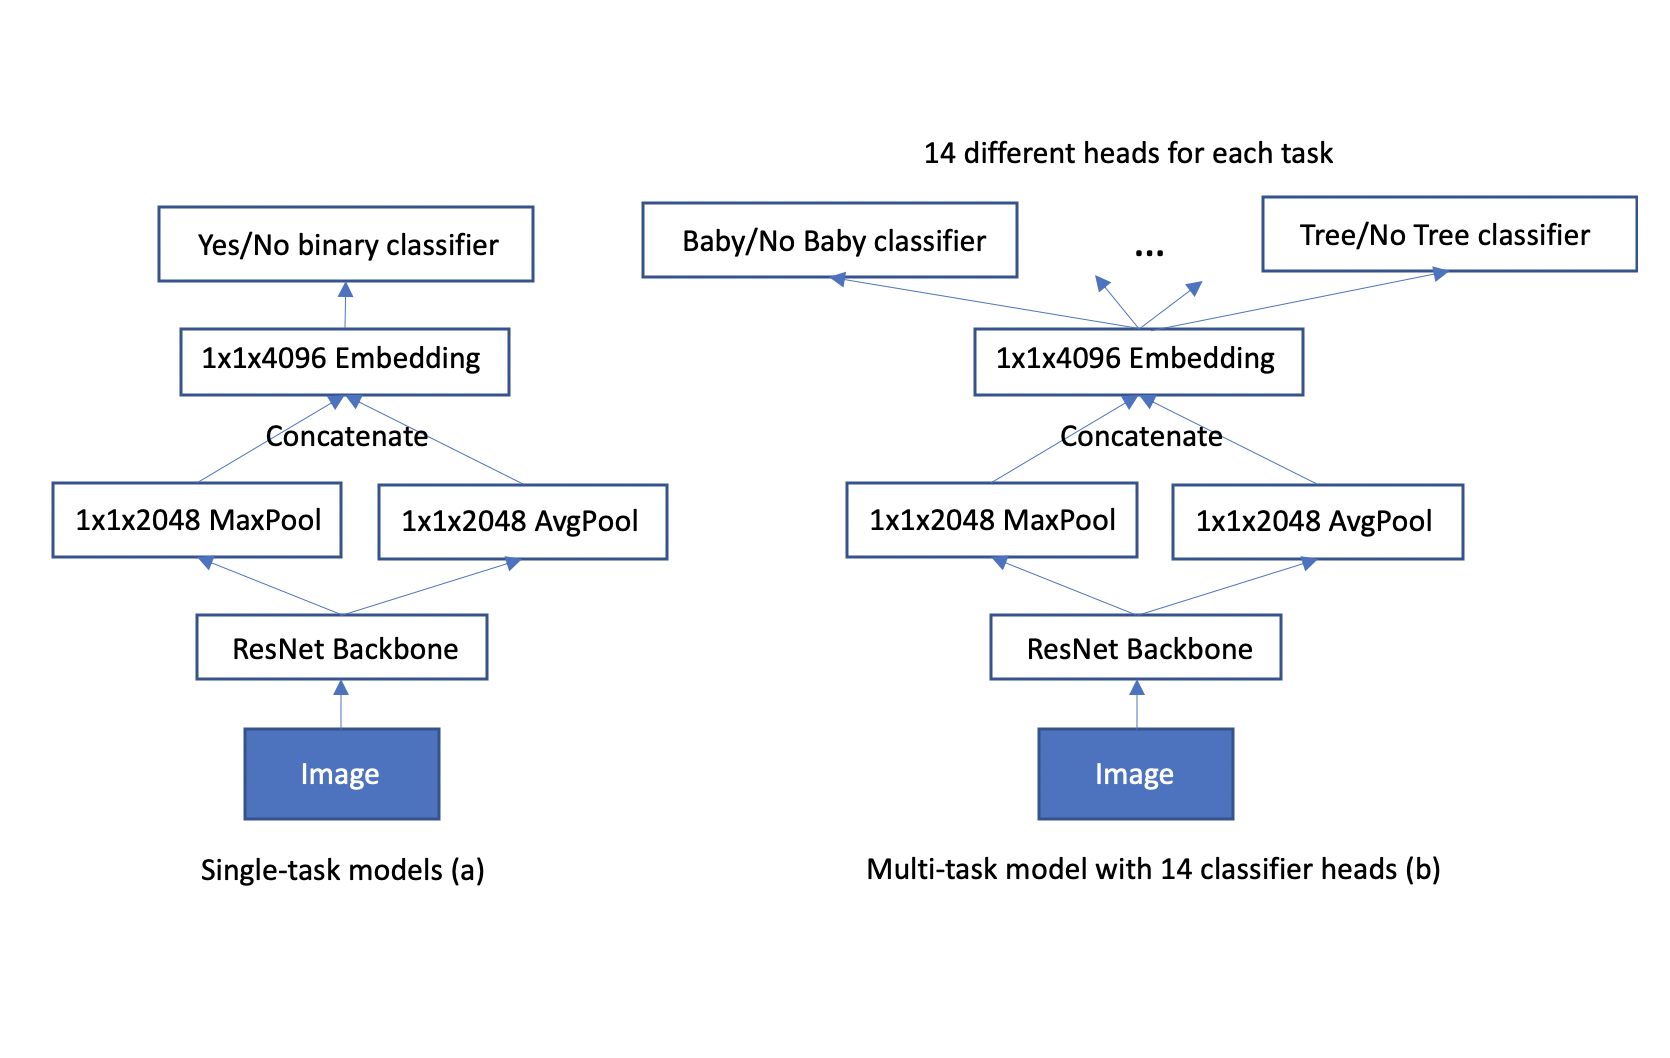
\includegraphics[width=0.8\textwidth]{imgs/image-labeling.png}
\caption{Architectures for both single-and multi-task models. The model (a) is the single-task model, which is the same for all 14 tasks. Model (b) is the Multi-task model, which contains 14 heads for each of the classification tasks. For these classifiers we took both max and average pool to create the embedding.}
\end{figure}

We will run some experiments on a 14 class multi-label prediction with some overlap between the classes in the images.
The 14 head multi-task model structure and the structure of the 14 identical single-task models are shown in Figure 6.3.
The goal here would be to see how what kind of a difference there would be in training with a single-task and multi-task model over all of the labels.

\begin{table}[]
    \centering
    \begin{tabular}{lccl}
        \multicolumn{1}{l}{\textbf{}}    & \multicolumn{1}{l}{\textbf{Multi-task}} & \multicolumn{1}{l}{\textbf{Single-task}} \\ \cline{2-3}
        \multicolumn{1}{l}{People} & \multicolumn{1}{c}{90\%}            & \multicolumn{1}{c}{89\%}                           \\ \hline
        \multicolumn{1}{l}{Man} & \multicolumn{1}{c}{87\%}               & \multicolumn{1}{c}{84\%}                        \\ \hline
        \multicolumn{1}{l}{Woman} & \multicolumn{1}{c}{86\%}               & \multicolumn{1}{c}{87\%}                           \\ \hline
        \multicolumn{1}{l}{Baby}       & \multicolumn{1}{c}{87\%}            & \multicolumn{1}{c}{93\%}                           \\ \hline
        \multicolumn{1}{l}{Sea}       & \multicolumn{1}{c}{89\%}               & \multicolumn{1}{c}{96\%}                        \\ \hline
        \multicolumn{1}{l}{River}       & \multicolumn{1}{c}{89\%}               & \multicolumn{1}{c}{88\%}                           \\ \hline
        \multicolumn{1}{l}{Bird} & \multicolumn{1}{c}{88\%}            & \multicolumn{1}{c}{89\%}                        \\ \hline
        \multicolumn{1}{l}{Car}       & \multicolumn{1}{c}{85\%}            & \multicolumn{1}{c}{94\%}                        \\ \hline
        \multicolumn{1}{l}{Clouds}       & \multicolumn{1}{c}{93\%}            & \multicolumn{1}{c}{93\%}                        \\ \hline
        \multicolumn{1}{l}{Dog}       & \multicolumn{1}{c}{87\%}            & \multicolumn{1}{c}{93\%}                           \\ \hline
        \multicolumn{1}{l}{Flower} & \multicolumn{1}{c}{85\%}            & \multicolumn{1}{c}{93\%}                        \\ \hline
        \multicolumn{1}{l}{Night}       & \multicolumn{1}{c}{87\%}            & \multicolumn{1}{c}{92\%}                        \\ \hline
        \multicolumn{1}{l}{Portrait}       & \multicolumn{1}{c}{89\%}            & \multicolumn{1}{c}{91\%}                        \\ \hline
        \multicolumn{1}{l}{Tree}       & \multicolumn{1}{c}{87\%}            & \multicolumn{1}{c}{92\%}                           \\ \hline
        \multicolumn{1}{l}{Average}       & \multicolumn{1}{c}{88\%}               & \multicolumn{1}{c}{91\%}                        \\ \hline
    \end{tabular}
    \caption{Accuracies on the data sets for both single-task and multi-task models. 
    The accuracy is the proportion for correct labelings in the balance evaluation set, so pure guess would result in 50\% accuracy.}
\end{table}

The dataset is a collection of 15000 images that have labels for some of the classes.
The number of labels for each task is highly varied.
The smallest tasks have dozens of images, whereas the largest ones have thousands.
From this dataset, we will take for each class a 15\% cut for validating the performance.
In this case, we will pose our main problem as a binary classification problem.
For each of the tasks, we will train a classifier telling if the label exists in the image or not.
The classifier will use a ResNet-101 as a backbone, and the head will be a regular fully connected layer connected to a positive and negative class for each of the tasks.
For the single-task models, we will have the same ResNet backbone as for the multi-task model.
The main metric that we will compare will be the ratio of correct labelings per class.
Since we pose this as a binary classification task, it is easy to guarantee that our test sets have an exact 50/50 split for positive and negative classes.
Similarly, while training, we can oversample the positive classes in a way to guarantee that each batch will have half positive and half negative classes.
This way, we won't learn classifiers that are biased toward predicting the absence of the label due to the small number of images for that class.
The control over the sampling of the data is a very beneficial trait of the multi-task problem setting.

To train the multi-task model, we experimented on various sampling ratios to find the best model.
Manually giving a meaningful sampling ratio is quite difficult due to the relatively large number of tasks in this multi-task model.
The various sampling ratios we tested for this data were equal sampling, data proportional sampling, and finally, some manual adjustments to the proportional sampling based on the results.
The proportional sampling was the one that produced the final best model.
It is quite an interesting result, considering just how small some of the classes are relative to the entire data set.
We tried adjusting the proportional ratios based on the difference from the single-task accuracies but could not find ratios that would have improved the performance.
Based on the previous results, we could say that there likely exists some ratios that could provide superior results, but finding them is too expensive.
With the best model, which was chosen based on the average accuracy on the validation data, the model achieved an average of 88\% accuracy in labeling all the tasks.
By average, we mean taking the accuracy of each task separately and averaging those averages and not the total ratio of correct classifications.

One new thing that we noticed when training on this data set was that with too high learning rates, the experiments were not very repeatable.
It seems that in a multi-task setting, it is not easy to tell that the learning rate is too high.
In this case, when the learning process seemed to progress in a manner that we would call expected, the learning rate might actually be too high.
With a slightly too high learning rate, it seemed like it is relatively random, whether the model reaches the best weights.
Most likely, the sampling ratios matter here quite a lot, but with the same sampling ratios and a slightly too high learning rate, there didn't seem to be a guarantee that anything close to the best model would be reached.
Maybe this has something to do with the large variance in the size of the datasets.
With more dynamic sampling ratios, the problems might solve themselves, as then some tasks would hopefully not get stuck at low accuracies.
We noticed here the same thing as in the leaves experiment that a long training process that slowly approaches the optimum seems to produce the best results in the end consistently.
Maybe this means that finding the intersection that can solve all the tasks optimally is relatively small and easy to overshoot with too large learning rates.
Similarly, with incorrect sampling ratios, the model would never be able to reach the weights needed for the shared optimal solution.

The single-task model training was done similarly to the multi-task model and by using the same data loading techniques.
This way, we reached an average accuracy of 91\%, beating the multi-task model slightly.
All the task-specific results for both multi- and single-task models are collected in Table 6.2.
Some part of the errors is due to the misclassification of the data, based on a random sample, around 2\% of the labels are wrong.
These results yet again show that it is possible to learn different tasks using the same representations.
Yes, in this case, the multi-task accuracy didn't match the single-task counterparts, but they are relatively close.
And all this is not really a fair comparison as the single-task models account for a total of around 14 times as many parameters.
If the single-task models were trained on significantly smaller backbones, the multi-task model could be more accurate, showing the benefit of using larger models over multiple tasks.
And even picking the smallest ResNets, the number of parameters over 14 tasks would be larger than a single ResNet101.

\section{Object detection}
In this section, we will use multiple data sources and combine them into a single powerful object detector.
To be specific, our goal is to create an object detector for 37 different cat and dog species.
The two datasets that we will use are the COCO dataset \citep{COCO} from which we will take the cat and dog classes and the Oxford-IIT Pet Dataset \citep{catsdogs}, which comprises of images with labels for the 37 different cat and dog species that we will detect.
In these experiments, the backbone used will be EfficientNet-0, which will be used in the EfficientDet architecture as well as an independent EfficientNet backbone.
The base for the code of the detector uses this Pytorch implementation of EfficientDet \citep{pytorch-efficientdet}.
The base model is then modified to meet the needs of our experiments.

There are multiple ways to approach this problem.
We will train two different models to see how the results differ.
The first approach is to do a brute-force two-stage detector, where we share the common backbone.
In this approach, the detector would try to learn to detect the dog and cat classes from the COCO dataset, while an object classifier is trained using the same backbone as the detector.
The object classifier is then responsible for giving the actual class of interest.
This way, the training is relatively simple, and the backbone would be used recursively.
Specifically, the detector would generate the regions for the animals that would be cropped and pushed through the backbone, this time to the classifier head.
This recursive use of the backbone is efficient in terms of the parameters, but running images through the same backbone twice could turn out to be too expensive as it would double the inference time.

\begin{figure}[h!] 
\centering 
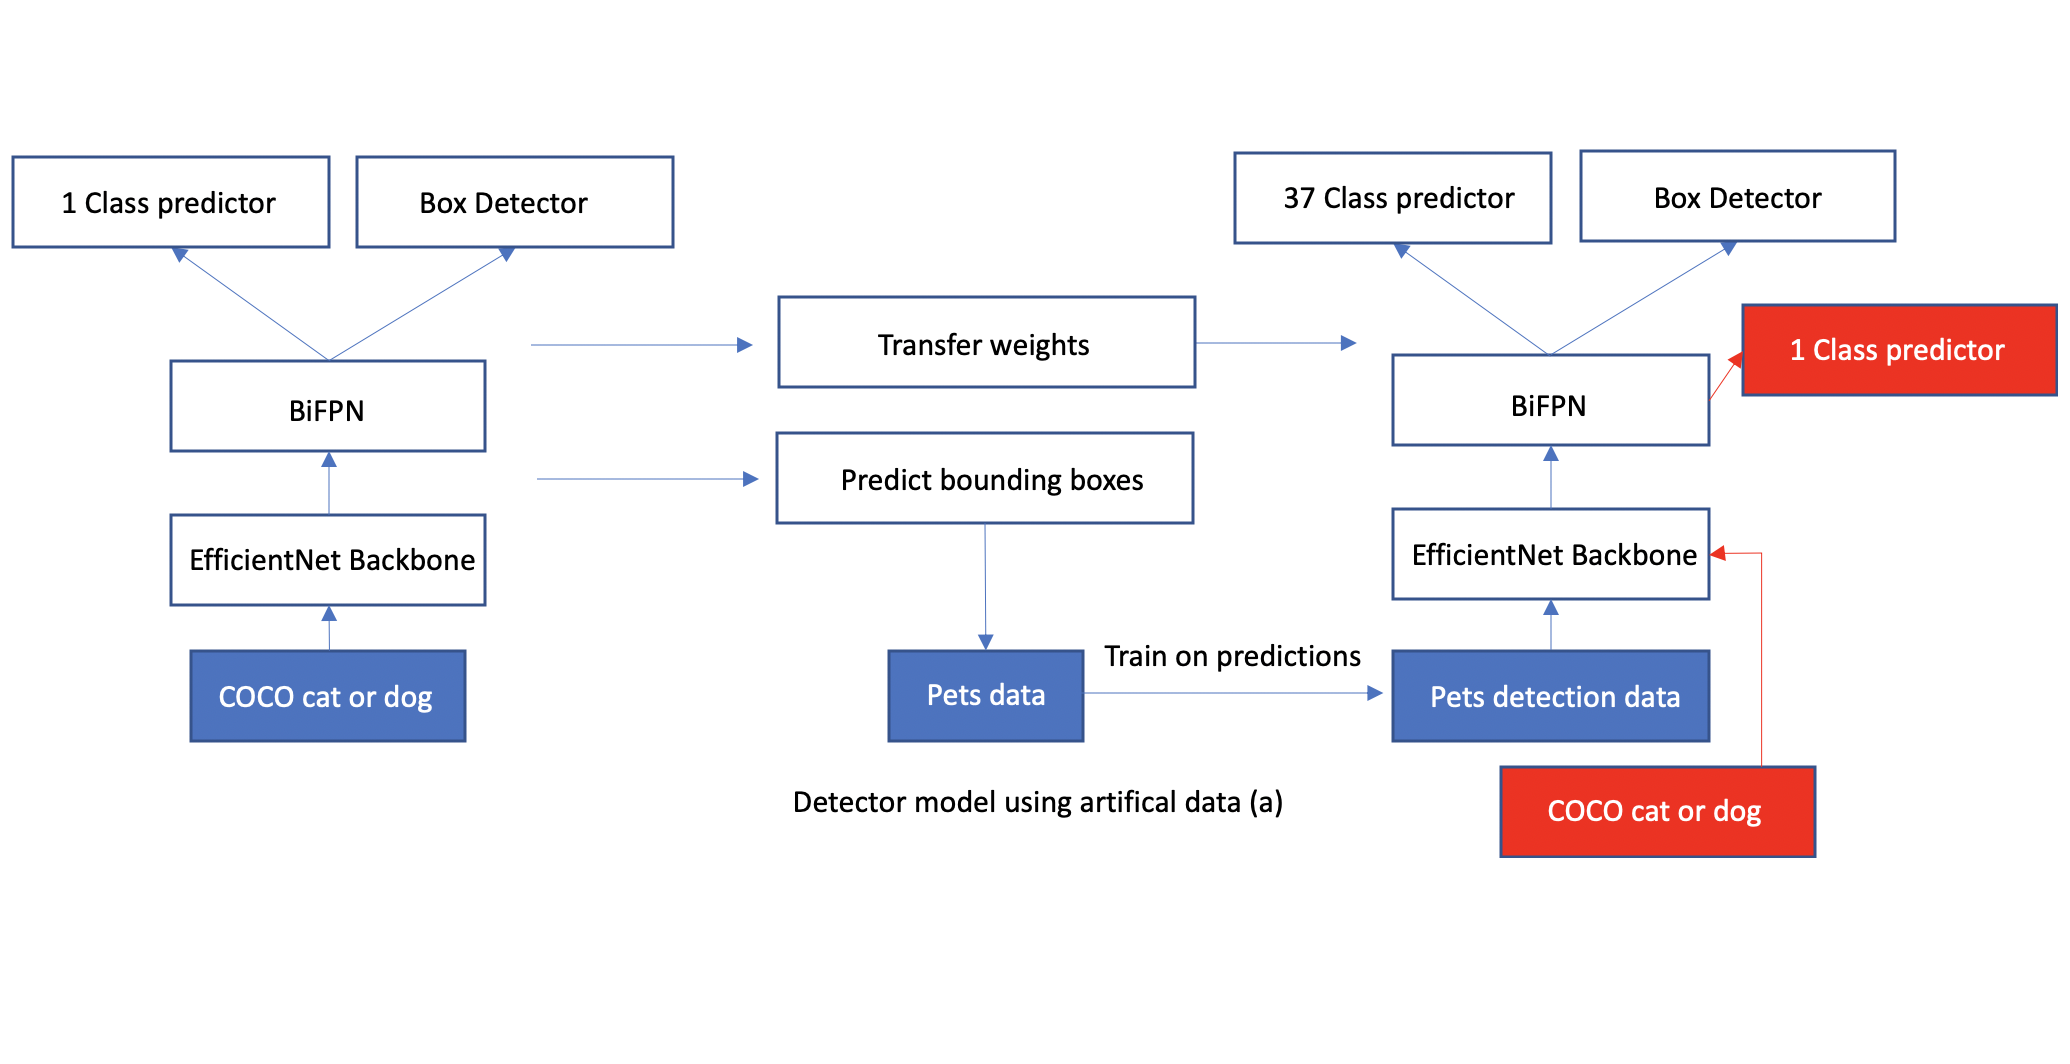
\includegraphics[width=0.8\textwidth]{imgs/object_detect_combine.png}
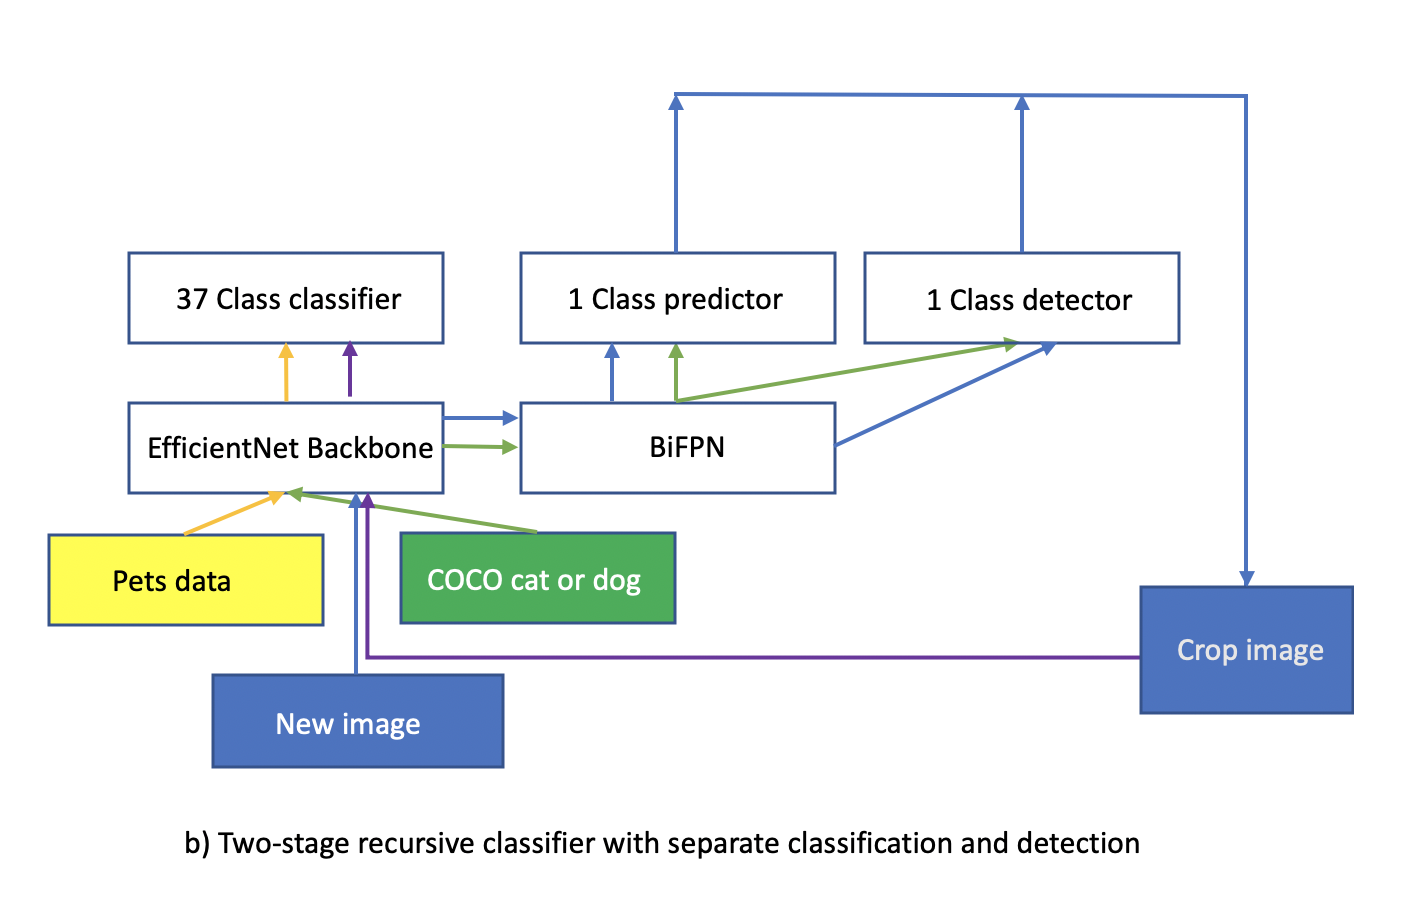
\includegraphics[width=0.8\textwidth]{imgs/recursive.png}
\caption{EfficientDet models for solving the object detection problem. In a), we have the basic object detector. We show how we train on the COCO data first and then transfer the weights to the model for the pets data with predicted bounding boxes. In red the additions needed to train on both the original data and artificially labeled are shown. Both tasks could share the weights for the detector but would need to have their own class head.  In b), we have the recursive object detector. In yellow, we describe the path to train on the pets data. With green, we describe the path to train the cat or dog object detector. In blue, we show the first cycle of a new prediction. With purple, we show the second cycle for the new detection.}
\end{figure}

The second way of approaching this problem is to first train a model on the COCO classes and to create a detector for the cat and dog classes.
Using the high-level model, we can automatically create acceptable object detection labels for the 37 classes in the pets dataset.
Then we can initialize a 37 class object detector using the weights of the two-class model.
By having such a well-initialized model for the detection, the second part of the training focuses on learning the features to differentiate between the very similar classes.
An interesting question here is just how well the object detector works when the classes are so similar.
In an image classifier setting, it would make sense that the model could learn the subtle features that are unique to each of the classes.
As we previously covered, the object detector is a multi-task problem. 
It follows that the network has to both decide the anchors most likely containing an object and also determining the class of the object.
If we look at the classes for the COCO dataset for object detection, for example, we can see that there are 80 classes, but they are relatively difficult to mix up due to being quite distinct from one another. 
In Figure 6.6, we have an example of two images from the pets dataset showing two classes that would be relatively easy to mix up.

\begin{figure}[h!] 
\centering 
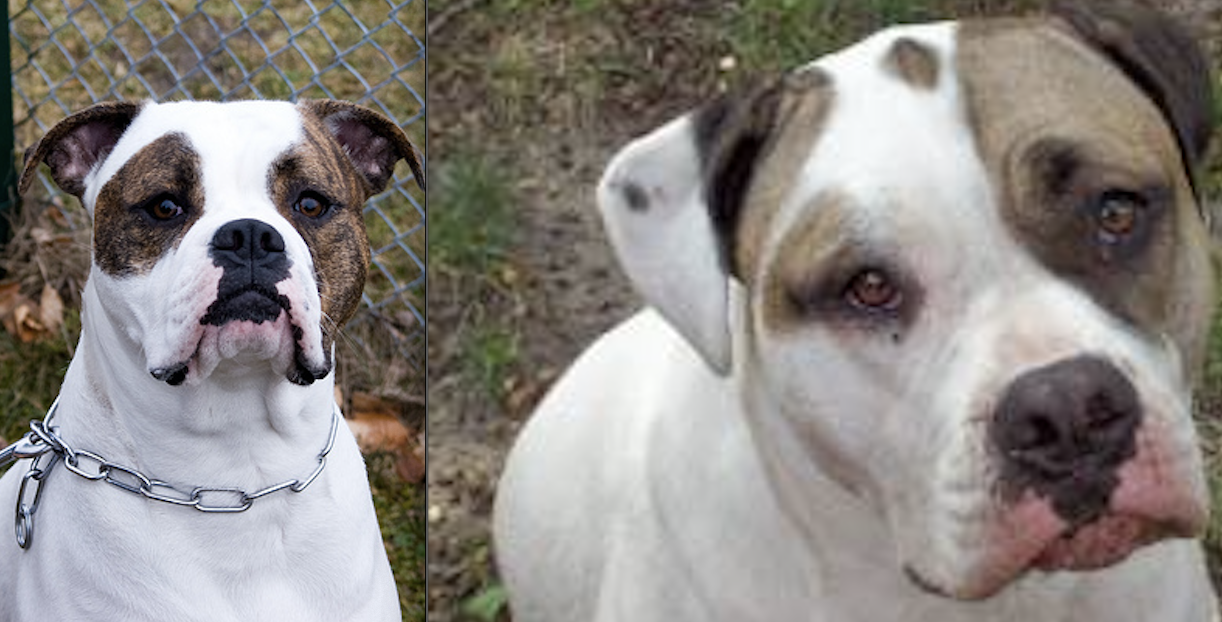
\includegraphics[width=0.8\textwidth]{imgs/pets-example.png}
\caption{Example of two very similar classes in the pets dataset. On the left is an American bulldog and on the right is an American pit bull terrier.}
\end{figure}

To evaluate the effects of both approaches, we will look at multiple metrics.
Since the two approaches are quite different, we can't make an entirely fair direct comparison between them.
To get somewhat of an idea for how well the models detect our 37 different classes, we will use a slightly arbitrary metric.
We will measure the accuracy of the detector on our test set for the pets dataset.
A positive example is one where the detector gives the highest confidence to the correct class.
This is a somewhat simplified version of measuring the detector performance.
The baseline scores for our EfficientNet-0 model are 92\% accuracy on the pets dataset and a 0.55 AP on detecting the cat and dog classes in the COCO dataset.
We will calculate these same scores for the recursive model to see how close the multi-task model can get.
To compare the two approaches, we will calculate the accuracy of correctly detected species in a set of the pets dataset.
The labels are not going to be perfect as they are generated by the model automatically, but should show if there are major discrepancies in the performance between the two approaches.

To train the single-stage model, we first created a new dataset in the COCO format from the dog and cat classes.
Instead of having two classes, we combined both dog and cat into a single category as the goal is to detect them as well as possible, and we are not interested in identifying whether it is a dog or a cat.
It is important to set the category id to be one instead of zero when training the object detector when there is only one class since otherwise, there will not be any predictions for the background.
With this new dataset, we initialized the EfficientDet model and trained it to detect the single class from the COCO dataset.
We first fine-tuned the head for ten epochs and then fine-tuned the entire network for 40 more epochs, and we picked the model with the lowest validation loss as the best one.
The chosen model achieved 0.54 AP when tested.
Then we created a new COCO style dataset out of the pets dataset.
To get the annotations, we ran the images through our one-class object detector and labeled all found boxes with the class of the image from the pets dataset.
The COCO format requires the labels as a tuple of four numbers signifying the x and y coordinates of the top left of the bounding box, followed by the bounding box width and the height.
Since most of the images in the pets dataset contain only a single animal, we could tell that there were incorrect boxes as the number of annotations was about 10-15\% higher than the number of images.
The bounding boxes were most likely not perfect, but good enough to get decent results.
We initialized the model with the weights of the original object detector, which meant that the regression loss for the model was consistently low.
So the training mostly focused on learning to minimize the classification loss with the new 37 classes.
Since this was a much more difficult problem than the original, it took a bit longer to reach the best model.
Evaluating the model on the artificial labels of the validation set gave an AP score of 0.55.

There are a few ways this kind of training could be extended to possibly get even better results.
We could attempt to train the largest possible model to get the best possible results on the original dataset so that the artificial labels for the unlabeled dataset would be the best possible.
We could create two heads in the object detector to train the detector on both the original COCO images and the new images in a multi-task setting to hopefully get a more general detector.
The training could get better if multiple cycles were completed, and the training would work in a semi-supervised way.
So what we used here would be the first labels for the new dataset.
The training would be done jointly on both datasets, as previously proposed.
Every n epochs, we would generate new bounding boxes for the pets dataset, to finally reach the optimal bounding boxes for the classes in the pets dataset.
Finally, we could do the label transfer also in the other direction.
Since the COCO has the correct bounding boxes, we could run the image classifier trained on the pets dataset on those boxes to generate the actual animal species for them.

The recursive model heavily relies on sharing the EfficientNet backbone in the detector between the classifier head and the detector head.
The model is recursive because, on the first pass, we will find the cat or dog regions from the model using the detector head.
Thus, the detector head is predicting only a single class as the distinction between the cat or dog class is of no interest in the detector.
Given these detected objects, we can crop them from the original image and pass through the other head, which is concerned with classifying the image into the 37 classes of interest.

For the recursive two-phase model, we trained it in a very similar fashion to the previous multi-task models.
In this case, we ran the experiment with only a few sampling ratios, of which a 50/50 split produced the best results.
The object detector only required adding the final classification head on top of the backbone, and then the model could be trained with a basic multi-task training loop since the EfficientNet backbone that we wanted to use is already a part of the EfficientDet model.


\begin{table}[]
    \centering
    \begin{tabular}{lccl}
        \multicolumn{1}{l}{\textbf{Pets classification}}    & \multicolumn{1}{l}{\textbf{}}  \\ \cline{1-2}
        \multicolumn{1}{l}{EfficientNet-B0 baseline} & \multicolumn{1}{c}{93\%}                    \\ \hline
        \multicolumn{1}{l}{Recursive detector task head}       & \multicolumn{1}{c}{89\%}                       \\ \hline
        \\
    \end{tabular}
    \caption{
    This table lists the accuracy for pets classification without localisation based on the baseline model and the classifier head in the recursive model.
    }
\end{table}


\begin{table}
    \centering
    \begin{tabular}{lccl}
        \multicolumn{1}{l}{\textbf{Cat or dog detection}}    & \multicolumn{1}{l}{\textbf{}}  \\ \cline{1-2}
        \multicolumn{1}{l}{EfficientDet-D0 baseline} & \multicolumn{1}{c}{0.54}                       \\ \hline
        \multicolumn{1}{l}{Recursive detector}       & \multicolumn{1}{c}{0.52}                    \\ \hline
    \end{tabular}
    \caption {
        This contains the AP score for detecting the single cat or dog class for the baseline and the recursive detector.    
    }
\end{table}
\begin{table}
    \centering
    \begin{tabular}{lccl}
        \multicolumn{1}{l}{\textbf{Custom pets detection metric}}    & \multicolumn{1}{l}{\textbf{}}  \\ \cline{1-2}
        \multicolumn{1}{l}{EfficientDet-D0 trained with artificial data} & \multicolumn{1}{c}{85\%}     \\ \hline 
        \multicolumn{1}{l}{Recursive detector with separate heads}       & \multicolumn{1}{c}{91\%}                       \\ \hline
    \end{tabular}
    \caption {
        This table compares the EfficientDet trained on artificial data and the recursive model in detecting the 37 pets classes.
        Here the metric is the proportion of correct classifications in the most confidently detected box.
    }
\end{table}
\begin{table}
    \centering
    \begin{tabular}{lccl}
        \multicolumn{1}{l}{\textbf{37 class object detection}}    & \multicolumn{1}{l}{\textbf{}}  \\ \cline{1-2}
        \multicolumn{1}{l}{EfficientDet-D0 artificial data 37 classes AP} & \multicolumn{1}{c}{0.55}                       \\ \hline
    \end{tabular}
    \caption {
        The AP score on 37 class object detection for the model with artificial data.
    }
\end{table}

To compare the models, we have collected the various metrics in Tables 6.3 to 6.5, grouped by the comparable metrics. 
The pure object detector for 37 classes had a 0.55 AP score on the artificially labeled dataset of the pets, and this is mildly higher than the base AP for the cat or dog detector.
While the number seems impressive given the number of highly similar classes, it is not exactly comparable to the baseline due to the fact that the pets dataset is not that varied in terms of having many or different sized animals.
Furthermore, the bounding box labels are created by the initial state of the 37 object detector, which likely causes the accuracy for the bounding boxes is going to be very high.
The regression loss of localizing the boxes stays very low and stable throughout all of the training, showing that likely the detection part does not change that much.
In our artificial detection evaluation metric, this pure detector achieved an 85\% accuracy.
The accuracy is relatively high, given the difficulty of detecting and classifying such similar classes.

The recursive multi-task model reached again slightly lower accuracies than the single task counterparts.
The AP score on the cat or dog detection task dropped by 0.02, and the accuracy on the pets classification dropped by 4\% to 89\%.
Interestingly, the detector task had a higher accuracy than the classification head had on the pets test set.
The better accuracy could result from the fact that classifying a cropped animal is easier than to classify it within a larger frame.
And since the object detector is relatively decent at finding the cat or dog candidates as a combination, these achieve better results.

Based on the numbers, we could say that the two-stage detector seems to be the better one.
The main downside to doing the two-stage detection is the fact that it would have to work one frame behind the video.
Since on the first loop, we would detect our objects in the first frame.
On the second frame, we would pass the second frame and the cropped images that we found in the first frame.
If the classification is done in this manner, the inference time cost won't be that much as it will be just the head to get the classification outputs.
In the case that multiple videos would be run in parallel, this could possibly not be possible as at some point, the input could be too large to handle as a single batch.
On the other hand, the pure detector doesn't need such considerations.
The pure detector's problem is that it has some obvious downsides due to the artificial training set that was created for it.
Whereas the recursive model does relatively as well on all kinds of data, the pure detector seems to have issues when there are multiple objects to detect, or the size varies.
These issues likely stem from the fact that the pets dataset consists mostly of single relatively large animals, which is not always the case.
Because the training and test sets are from the same source, they are relatively similar, so the performance is very transferable between those tasks.
Some of the previously mentioned ways of training could alleviate this problem.
Perhaps by having two classifier heads and doing auxiliary training on the COCO cats and dogs could make the detector detect the animals better, and hopefully, the classifier could solve the problem for all sizes from the single source.
This modification is also pictured in Figure 6.4.

\section{Detection, classification and segmentation}
Thinkkers do it like it is done in \citep{multinet} but use efficientnet for all parts?

\section{Recap}
This will be an overview of all the challenges and things about multi-task training based on the experiments we have done.
\chapter{Conclusions}
Do some final review on why multi-task learning is a good idea given the problems shown and some personal experiments and what are the problems it brings.
Show how a multi-task setting is a trade-off between inference time and training time difficulty to motivate when it is a good idea or not.
% \chapter{Introduction}
\section{Problem statement and motivation}
The following gives some superficial instructions for using this template for a Master's thesis. For guidelines on thesis writing you can consult various sources, for example, the Bachelor thesis template.

The thesis should have an introduction chapter. Other chapters can be named according to the topic. In the end, some summary chapter is needed; see Chapter~\ref{chapter:conclusions} for an example.

\section{Structure of thesis}
Cool stuff etc.

\chapter{Neural networks}
Background stuff 
\section{Fully Connected Networks}
When needed, when good/bad
\section{Convolutional Neural Networks}
Show some basic CNN things maybe
\subsection{Neural image processing}
How it different from classical features and how it works
\section{Attention}
Attention huh
\section{Multi-task learning}
Describe how a multi-task setting differs
\section{RNN/LSTM/Transformer text processing/generation}
Depending on what may be used

\chapter{Tasks}
What has been done when solving these tasks/history/formal definition
\section{Image classification}
Image classification is one of the basic modern computer vision problems, where the goal is to create a model that can classify an input image into one of a set of pre-defined classes. Prior to the popularization of applying large Convolutional Neural Networks for this task, the most successful way of solving the problem was to use some algorithm for finding feature descriptors in a set of images and then training a linear classifier, like a Support Vector Machine over a Visual Bag of Words representation of the images. These days nearly all approaches are based on using deep CNNs.
\subsection{ImageNet}
ImageNet  \citep{imagenet}  is perhaps the most significant dataset for image classification and especially the ImageNet Challenge \citep{ILSVRC}, which is a challenge for a collection of 1000 classes from the ImageNet dataset for image classification using 1.2 million training and 150 thousand  images of the entire ImageNet dataset. In 2012 the winning model, AlexNet \citep{alexNet}, showed that it was possible to train a deep CNNs efficiently using GPUs. Since 2012 all top-performing models showed some new improvements on how to create the most performant network architecture, for example, VGGNet from the year 2014 and ResNet \citep{resNet} from 2015, both of which have been popular models to use for Transfer Learning since.

Human accuracy on the ImageNet challenge is about 5.1\% \citep{imageNet_summary}, and ResNet achieves a top-5 error rate of 3.57\% \citep{resNet} and newer architectures even lower, but this still does not mean that image classification is a solved problem. The human performance experiment found that many of the human errors are caused by not having expert information in, for example, identifying animal species or not even being aware of the existence of a class \citep{imageNet_summary}. ObjectNet \citep{objectNet} is a dataset designed to  image classifiers with a focus on their generalizability. It contains many classes that also exist in the ImageNet dataset. However, they are in unexpected locations or have an unexpected pose, causing the high accuracy image classifiers trained on ImageNet experience a 40-45\% accuracy drop when evaluating them on the ObjectNet images of classes shared between ImageNet and ObjectNet. This kind of adjustment is relatively easy for a human, and it shows that while the classifiers are good, they are by no means perfect.
\subsection{Transfer learning}
Unlike the ImageNet challenge, most real-world tasks do not have such an abundance of data for all possible classes. Still, to achieve the highest accuracies, they require models that are equal in terms of complexity to those that have top accuracies problems on the scale of the ImageNet classification. For this reason, many CNN classifiers, irrespective of the problem, feature one of the ImageNet classifiers or similar as a backbone to solve a part of the problem. Even though some datasets may contain a large number of images per class, using a pre-trained classifier as a basis often produces a better final classifier by applying fine-tuning \citep{betterTransfer}.

The idea behind transfer learning is to train on a related task to the end task first. Then the network weights in the model for the actual task are initialized to those of the model we are transferring from, so the training of the original model is a pre-step to the real task. Since training the models on ImageNet scale datasets is not generally feasible due to their large number of parameters and long training time, one of the pre-trained models is picked and then fine-tuned. Fine-tuning a classifier means taking the examples for the final task, and training the network on those, updating the original classifier at the same time. This differs greatly from the traditional learning model where each task is considered to be a separate model that has to be learned from scratch.

\begin{figure}[h!] 
\centering 
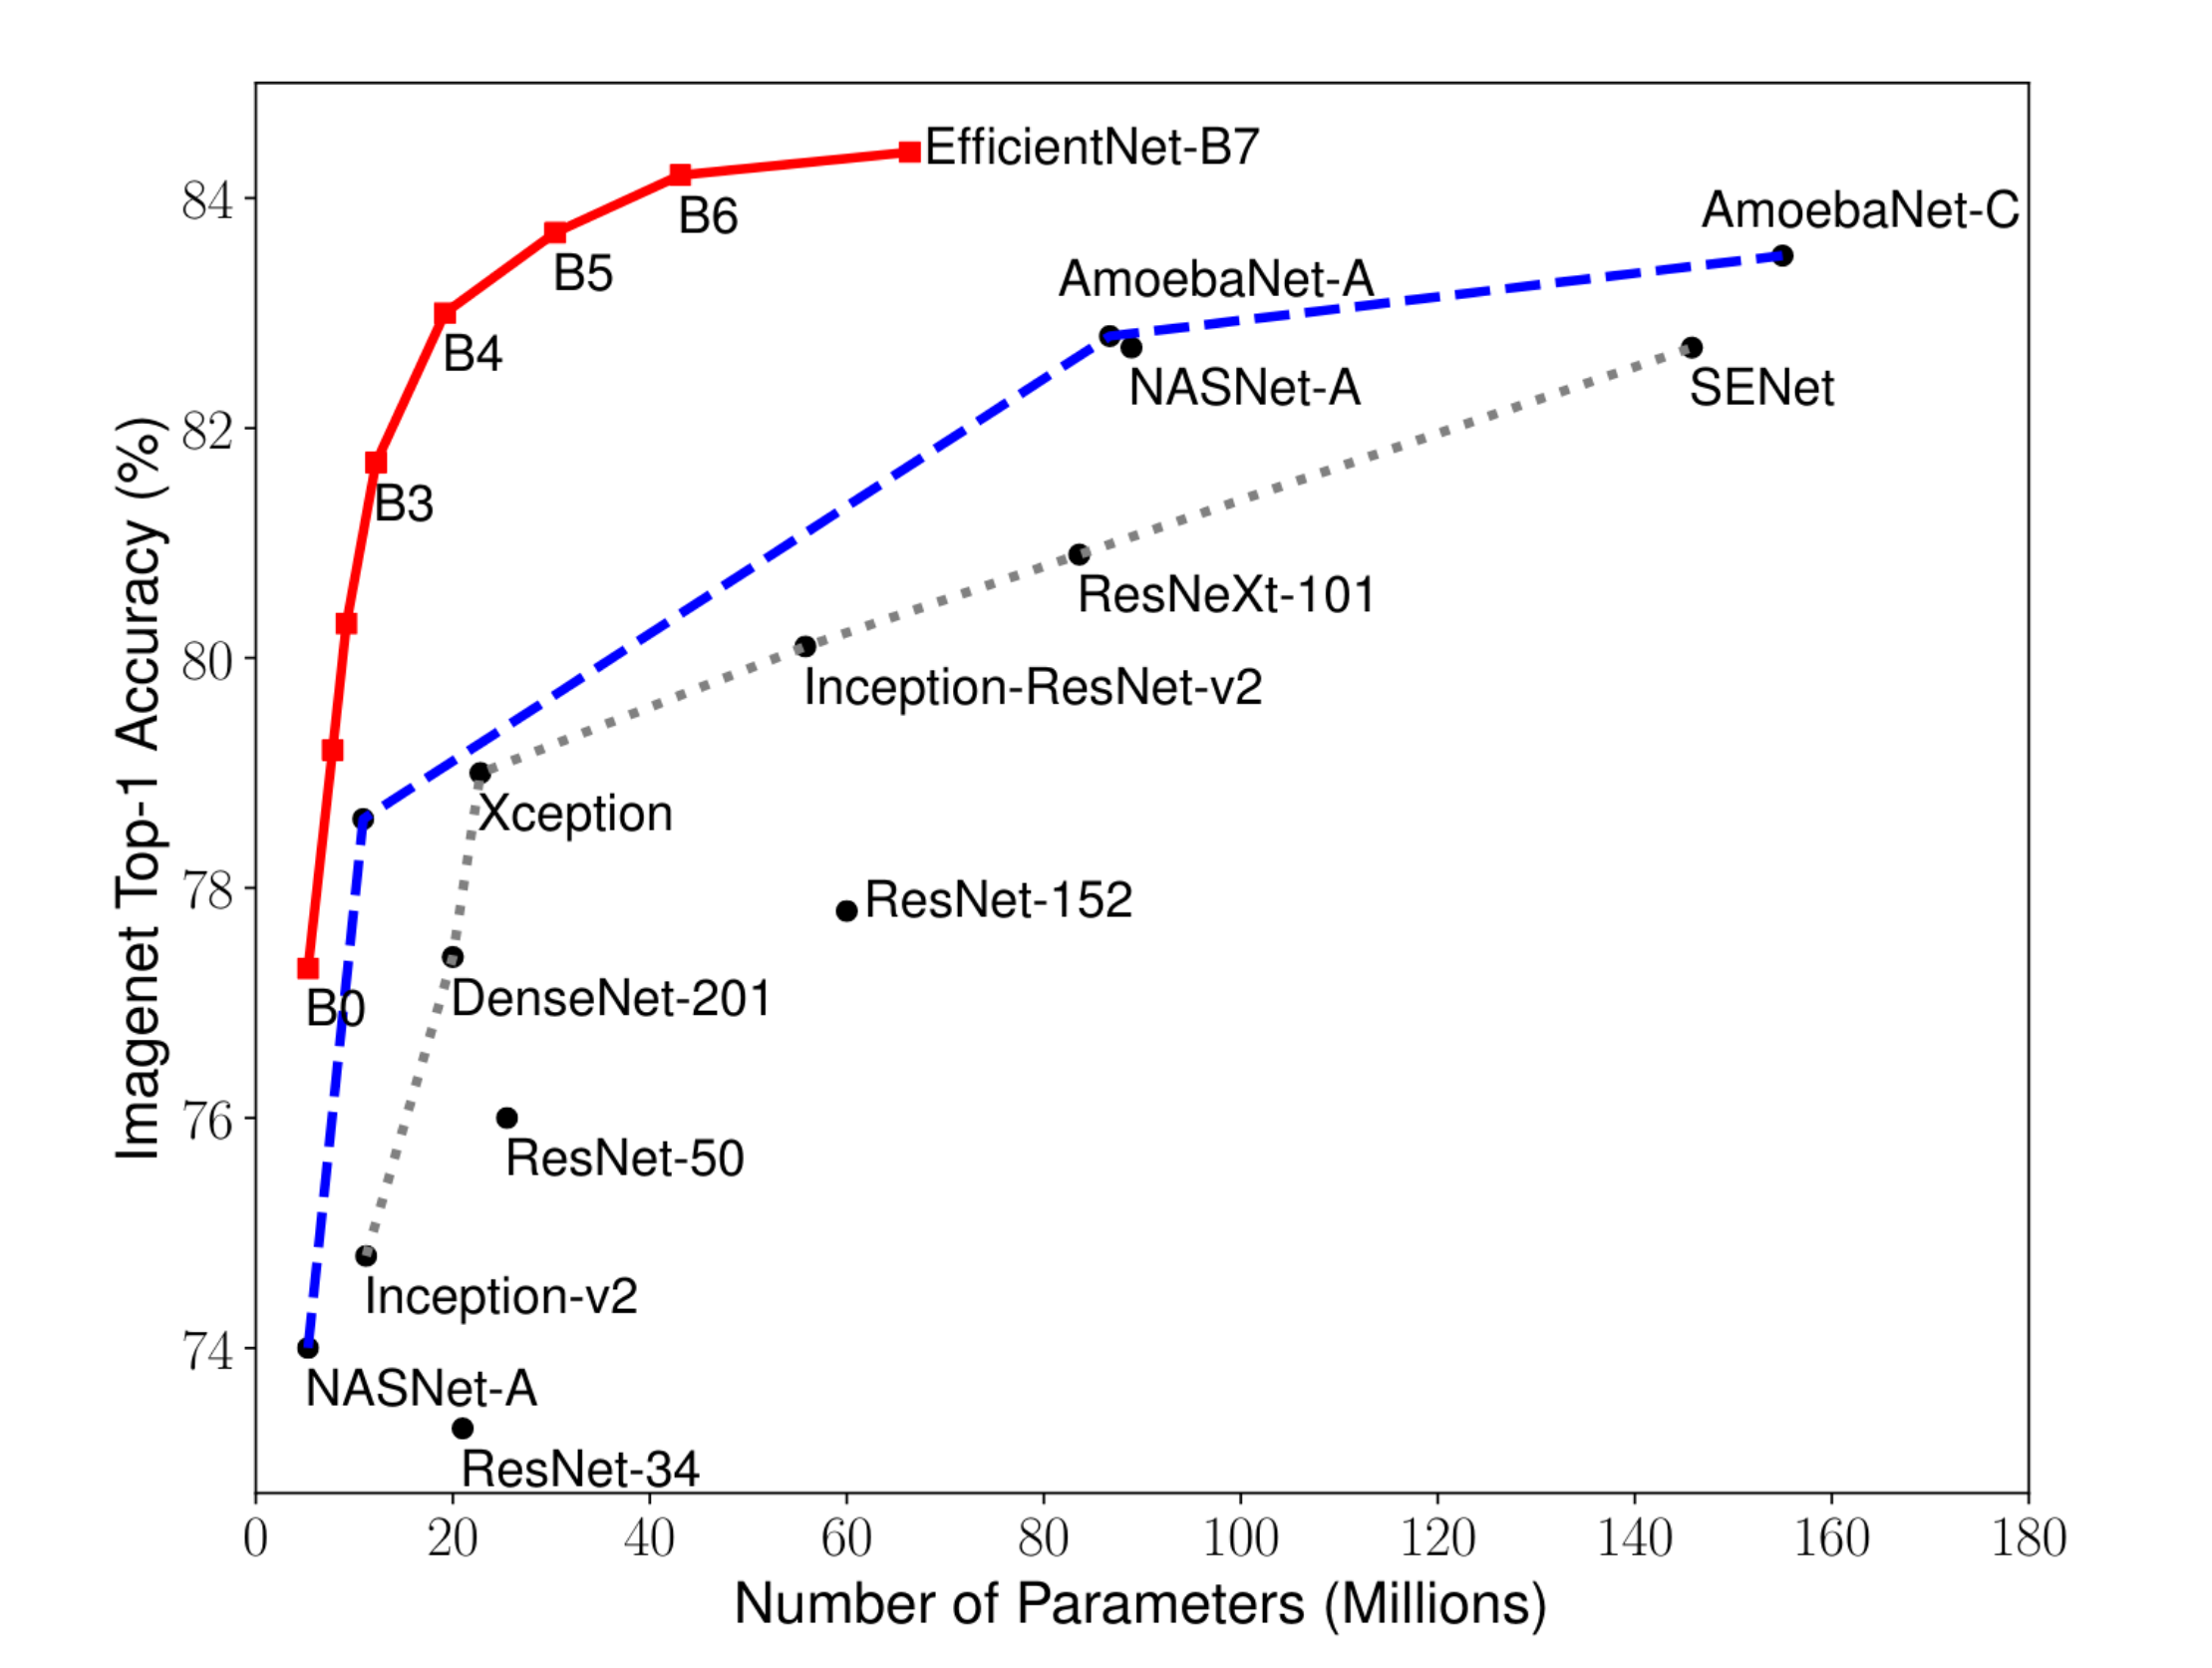
\includegraphics[width=0.8\textwidth]{imgs/imagenet_parameters.png}
\caption{Number of parameters in popular ImageNet classifiers. Figure from \citep{efficientNet}.\label{fig:params}}
\end{figure}

Picking which classifier to use as a base is often problem-dependent. As it is not possible to declare one network structure to be the best at all tasks, picking the best model to start with usually requires the user to compare different architectures and weighing the requirements for the problem at hand. Often though, the larger models will perform better, and there exists a correlation between performing well on ImageNet and being a good transfer learning model \citep{betterTransfer}. Though as can be seen in figure 3.1, better performance often comes at the cost of many more parameters, requiring more memory to train the model. Though just the number of parameters is not the only thing to compare as the throughput of a Resnet50 turns out to be about three times as large as the throughput of an EfficientNet-B4 even though they have a similar amount of parameters \citep{classifierPerformance}.

To formally define transfer learning, let $\mathcal{D}$ be a domain for the features, in this case, images.
\subsection{ResNet}
\subsection{EfficientNet}
\section{Object detection}
Based on what is going to be detected, maybe text?
\section{Paragraph captioning}
Assuming we are doing this
\section{Multi task learning}
Cover some examples of MTL in Computer Vision

\chapter{Datasets}
Describing our data
\section{Data formats}
Describe what datasets are used for each of the tasks and where they are from etc.

\chapter{Experiments}
Here are our experiments
\section{Training process}
\subsection{Evaluation criterias}
eval
\section{Image classifiers}
Results of image classsifiers on the datasets maybe compare ResNet vs EfficientNet
\subsection{Only transfer learned classifier}
Just a ResNet or something
\subsection{Image classifier with attention}
Add attention to image classifier
\subsection{Classifiers combined to a multi-task model}
How it do
\section{Object detection}
Some stuff for object detection
\section{Multi-task models}
Create multi-task models for all and try to find some pairs/tuples that actually work together properly
\chapter{Result analysis}
Incredible models absolutely.

\chapter{Future work}
How to make it better what could be tried 

\chapter{Figures and Tables}

\section{Figures}
Figure~\ref{fig:logo} gives an example how to add figures to the document. Remember always to cite the figure in the main text.

\begin{figure}[h!] 
\centering 

\includegraphics[width=0.3\textwidth]{HY-logo-ml.png}
\caption{University of Helsinki flame-logo for Faculty of Science.\label{fig:logo}}
\end{figure}

\section{Tables}

Table~\ref{table:results} gives an example how to report experimental results. Remember always to cite the table in the main text. 

\begin{table}
\centering
\caption{Experimental results.\label{table:results}}
\begin{tabular}{l||l c r} 
Experiment & 1 & 2 & 3 \\ 
\hline \hline 
$A$ & 2.5 & 4.7 & -11 \\
$B$ & 8.0 & -3.7 & 12.6 \\
$A+B$ & 10.5 & 1.0 & 1.6 \\
\hline
%
\end{tabular}
\end{table}

\chapter{Citations}

\section{Citations to literature}

References are listed in a separate .bib-file. In this case it is named \texttt{bibliography.bib} including the following content:
\begin{verbatim}
@article{einstein,
    author =       "Albert Einstein",
    title =        "{Zur Elektrodynamik bewegter K{\"o}rper}. ({German})
        [{On} the electrodynamics of moving bodies]",
    journal =      "Annalen der Physik",
    volume =       "322",
    number =       "10",
    pages =        "891--921",
    year =         "1905",
    DOI =          "http://dx.doi.org/10.1002/andp.19053221004"
}
 
@book{latexcompanion,
    author    = "Michel Goossens and Frank Mittelbach and Alexander Samarin",
    title     = "The \LaTeX\ Companion",
    year      = "1993",
    publisher = "Addison-Wesley",
    address   = "Reading, Massachusetts"
}
 
@misc{knuthwebsite,
    author    = "Donald Knuth",
    title     = "Knuth: Computers and Typesetting",
    url       = "http://www-cs-faculty.stanford.edu/%7Eknuth/abcde.html"
}
1
\end{verbatim}

In the last reference url field the code \verb+%7E+ will translate into \verb+~+ once clicked in the final pdf.

References are created using command \texttt{\textbackslash cite\{einstein\}}, showing as \citep{einstein}. Other examples: \citep{latexcompanion,knuthwebsite}.

Citation style can be negotiated with the supervisor. See some options in \url{https://www.sharelatex.com/learn/Bibtex_bibliography_styles}.

\section{Crossreferences}

Appendix~\ref{appendix:model} on page~\pageref{appendix:model} contains some additional material.

\chapter{From tex to pdf}

In Linux, run \texttt{pdflatex filename.tex} and \texttt{bibtex filename.tex} repeatedly until no more warnings are shown. This process can be automised using make-command.
 
\chapter{Conclusions\label{chapter:conclusions}}

It is good to conclude with a summary of findings. You can also use separate chapter for discussion and future work. These details you can negotiate with your supervisor.

%%%%%%%%%%%%%%%%%%%%%%%%%%%%%%%%%%%%%%%%%%%%%%%%%%%%%%%%%
\cleardoublepage                          %fixes the position of bibliography in bookmarks
\phantomsection
\addcontentsline{toc}{chapter}{\bibname}  % This lines adds the bibliography to the ToC
\printbibliography

%%%%%%%%%%%%%%%%%%%%%%%%%%%%%%%%%%%%%%%%%%%%%%%%%%%%%%%%%
\backmatter
\begin{appendices}

\end{appendices}
%%%%%%%%%%%%%%%%%%%%%%%%%%%%%%%%%%%%%%%%%%%%%%%%%%%%%%%%%

\end{document}
